% =============================================================================
% AVGO Equity Research Report
% Washington Square Research Partners (NYU MSFE)
% Tanishk Yadav | Martin Baretto | Ramana Sriram
% Version 2: BUY rating, Bloomberg-tearsheet cover
% =============================================================================
\documentclass[10pt,letterpaper]{article}

\usepackage[margin=0.85in,top=1.0in,bottom=0.95in]{geometry}
\usepackage[T1]{fontenc}
\usepackage{xcolor}
\usepackage{amsmath}
\usepackage{amssymb}
\usepackage{graphicx}
\usepackage{booktabs}
\usepackage{colortbl}
\usepackage{tabularx}
\usepackage{array}
\usepackage{multicol}
\usepackage{multirow}
\usepackage{fancyhdr}
\usepackage{titlesec}
\usepackage[hidelinks]{hyperref}
\usepackage{caption}
\usepackage{enumitem}
\usepackage{setspace}
\usepackage{tikz}
\usepackage{float}
\usetikzlibrary{positioning,calc}

% NYU palette
\definecolor{nyuviolet}{HTML}{57068C}
\definecolor{nyulight}{HTML}{8900E1}
\definecolor{nyudark}{HTML}{330050}
\definecolor{nyugrey}{HTML}{404040}
\definecolor{nyulgrey}{HTML}{D8D8D8}
\definecolor{accentgold}{HTML}{C99700}
\definecolor{accentgreen}{HTML}{0E7C3A}
\definecolor{accentred}{HTML}{A4123F}
\definecolor{rowshade}{HTML}{F2EAFB}
\definecolor{tickerblack}{HTML}{0C0C18}
\definecolor{tickergrey}{HTML}{1F1F2E}

% Page style
\pagestyle{fancy}
\fancyhf{}
\fancyhead[L]{\raisebox{-0.15\height}{
\includegraphics[height=12pt]{logo_small.png}} \hspace{2pt} \color{nyuviolet}\bfseries\small Broadcom Inc. (AVGO) \textbar{} Equity Research}
\fancyhead[R]{\color{nyugrey}\small 25 April 2026 \textbar{} \textbf{BUY} \textbar{} PT \$475}
\fancyfoot[L]{\color{nyugrey}\footnotesize Washington Square Research Partners \textbar{} NYU MSFE}
\fancyfoot[R]{\color{nyugrey}\footnotesize Page \thepage}
\renewcommand{\headrulewidth}{0.6pt}
\renewcommand{\headrule}{{\color{nyuviolet}\hrule width\headwidth height\headrulewidth}\vskip-\headrulewidth}
\renewcommand{\footrulewidth}{0.3pt}

% Section formatting
\titleformat{\section}{\Large\bfseries\color{nyuviolet}}{\thesection.}{0.5em}{}[{\color{nyulgrey}\titlerule[1pt]}]
\titleformat{\subsection}{\large\bfseries\color{nyudark}}{\thesubsection}{0.5em}{}
\titleformat{\subsubsection}{\normalsize\bfseries\color{nyudark}}{\thesubsubsection}{0.5em}{}
\titlespacing{\section}{0pt}{14pt}{6pt}
\titlespacing{\subsection}{0pt}{10pt}{4pt}

% Caption styling
\captionsetup{font=small,labelfont={bf,color=nyuviolet},labelsep=period}

\setlength{\parskip}{4pt}
\setlength{\parindent}{0pt}
\renewcommand{\arraystretch}{1.20}

% Byline command for each section
\newcommand{\sectionbyline}[2]{%
\begin{flushright}\vspace{-0.6em}%
{\footnotesize\color{nyugrey}\textit{#1 \textbar{} #2}}%
\end{flushright}\vspace{-0.4em}}

\begin{document}

% =============================================================================
% COVER PAGE — BLOOMBERG TEARSHEET STYLE
% =============================================================================
\thispagestyle{empty}
\newgeometry{margin=0in,top=0in,bottom=0in}

\begin{tikzpicture}[remember picture,overlay]

% --- Top white band with firm logo (logo_big.png) ---
\fill[white] (current page.north west) rectangle ([yshift=-0.85in]current page.north east);
\node[anchor=north west,inner sep=0pt]
  at ([xshift=0.6in,yshift=-0.22in]current page.north west)
  {
\includegraphics[height=0.22in]{logo_small.png}\hspace{6pt}
\includegraphics[height=0.42in]{logo_big.png}};

% Date / identifier right-aligned in the white band
\node[anchor=north east,text=nyugrey,font=\fontsize{10}{12}\sffamily,inner sep=0pt]
  at ([xshift=-0.6in,yshift=-0.28in]current page.north east) {25 April 2026};
\node[anchor=north east,text=nyugrey,font=\fontsize{9}{11}\sffamily,inner sep=0pt]
  at ([xshift=-0.6in,yshift=-0.46in]current page.north east) {Sector: Technology};
\node[anchor=north east,text=nyugrey,font=\fontsize{9}{11}\sffamily,inner sep=0pt]
  at ([xshift=-0.6in,yshift=-0.60in]current page.north east) {Industry: Semiconductors \& Software};
\node[anchor=north east,text=nyudark,font=\fontsize{9}{11}\itshape,inner sep=0pt]
  at ([xshift=-0.6in,yshift=-0.74in]current page.north east) {NYU MSFE Equity Research \textbar{} Initiation of Coverage};

% --- Violet accent stripe ---
\fill[nyuviolet] ([yshift=-0.85in]current page.north west) rectangle ([yshift=-0.90in]current page.north east);

% --- Black band with Broadcom logo + ticker ---
\fill[tickerblack] ([yshift=-0.90in]current page.north west) rectangle ([yshift=-1.80in]current page.north east);

% Broadcom logo (left side of black band)
\node[anchor=north west,inner sep=0pt]
  at ([xshift=0.6in,yshift=-1.05in]current page.north west)
  {
\includegraphics[height=0.50in]{broadcom_logo.png}};

% Ticker text next to logo
\node[anchor=north west,text=white,font=\fontsize{30}{36}\bfseries,inner sep=0pt]
  at ([xshift=2.25in,yshift=-1.05in]current page.north west) {AVGO};
\node[anchor=north west,text=white!70,font=\fontsize{10}{12}\sffamily,inner sep=0pt]
  at ([xshift=2.25in,yshift=-1.45in]current page.north west) {NASDAQ \textbar{} BROADCOM INC \textbar{} USD};

% Price + change (right side of black band)
\node[anchor=north east,text=white,font=\fontsize{28}{34}\bfseries,inner sep=0pt]
  at ([xshift=-0.6in,yshift=-1.05in]current page.north east) {\$422.76};
\node[anchor=north east,text=accentgreen!70!white,font=\fontsize{11}{14}\bfseries\sffamily,inner sep=0pt]
  at ([xshift=-0.6in,yshift=-1.45in]current page.north east) {\(\blacktriangle\) +32.6\% (30D) \quad +121.6\% (12M)};

% --- Headline ---
\node[anchor=north west,text=tickerblack,font=\fontsize{24}{30}\bfseries,inner sep=0pt,text width=7.2in]
  at ([xshift=0.6in,yshift=-2.15in]current page.north west)
  {Six-customer XPU franchise + margin-stable AI ramp};
\node[anchor=north west,text=nyuviolet,font=\fontsize{14}{18}\bfseries,inner sep=0pt,text width=7.2in]
  at ([xshift=0.6in,yshift=-3.10in]current page.north west)
  {Initiating BUY \textbar{} 12-month PT \$475 \textbar{} +12\% upside};

% --- Recommendation ribbon (right side) ---
\fill[accentgreen] ([xshift=0.6in,yshift=-3.65in]current page.north west) rectangle ([xshift=2.6in,yshift=-4.25in]current page.north west);
\node[anchor=center,text=white,font=\fontsize{28}{32}\bfseries]
  at ([xshift=1.6in,yshift=-3.95in]current page.north west) {BUY};
\node[anchor=west,text=tickerblack,font=\fontsize{14}{18}\bfseries]
  at ([xshift=2.85in,yshift=-3.85in]current page.north west) {Target: \$475.00};
\node[anchor=west,text=nyugrey,font=\fontsize{10}{14}]
  at ([xshift=2.85in,yshift=-4.05in]current page.north west) {12-month horizon \textbar{} Dec-2026};
\node[anchor=west,text=accentgreen,font=\fontsize{12}{14}\bfseries]
  at ([xshift=2.85in,yshift=-4.23in]current page.north west) {Implied upside +12.3\%};

% =============================================================================
% Tearsheet body: 2-column layout below the header strip
% =============================================================================
% Left column - data tables (compact, stacked)
\node[anchor=north west,inner sep=0pt,text width=2.6in]
  at ([xshift=0.6in,yshift=-4.6in]current page.north west) {%
\renewcommand{\arraystretch}{1.0}\setlength{\tabcolsep}{3pt}%
{\color{nyuviolet}\rule{\linewidth}{0.5pt}}\\[-2pt]
{\scriptsize\bfseries\color{nyuviolet}MARKET DATA \& FY25A OPERATING}\\[-3pt]
{\color{nyuviolet}\rule{\linewidth}{0.3pt}}\\[1pt]
{\scriptsize
\begin{tabularx}{\linewidth}{@{}>{}X>{}r@{}}
Last price (24-Apr-26) & \$422.76 \\
52W range & \$138 -- \$423 \\
Market cap / EV & \$2.00T / \$2.05T \\
Diluted shares & 4{,}969 mn \\
Beta (5Y / 2Y) & 1.63 / 1.20 \\
Revenue / EBITDA & \$63.9B / \$43.2B \\
EBITDA margin / EPS & 67.7\% / \$6.82 \\
FCF / NetDebt-EBITDA & \$26.9B / 1.13$\times$ \\
\end{tabularx}}\\[4pt]
{\color{nyuviolet}\rule{\linewidth}{0.5pt}}\\[-2pt]
{\scriptsize\bfseries\color{nyuviolet}VALUATION TRIANGULATION}\\[-3pt]
{\color{nyuviolet}\rule{\linewidth}{0.3pt}}\\[1pt]
{\scriptsize
\begin{tabularx}{\linewidth}{@{}>{}X>{}r@{}}
DCF (5Y FCFF) & \$436 \\
SOTP (FY27E EV/EBITDA) & \$401 \\
Comps Fwd P/E (22$\times$) & \$440 \\
Comps EV/EBITDA (18$\times$) & \$409 \\
Monte Carlo median & \$456 \\
Street median (n=11) & \$477 \\
\rowcolor{rowshade}\color{nyuviolet}\textbf{Our 12M PT} & \textbf{\$475} \\
\end{tabularx}}\\[4pt]
{\color{nyuviolet}\rule{\linewidth}{0.5pt}}\\[-2pt]
{\scriptsize\bfseries\color{nyuviolet}KEY CATALYSTS (NEXT 12M)}\\[-3pt]
{\color{nyuviolet}\rule{\linewidth}{0.3pt}}\\[2pt]
{\scriptsize
\begin{tabularx}{\linewidth}{@{}>{}p{0.65in} X@{}}
5-Jun-2026  & Q2 FY26 earnings \\
H2-2026     & TPU 3nm vol.\ ramp \\
H2-2026     & OpenAI rack ship \\
4-Sep-2026  & Q3 FY26 earnings \\
Dec-2026    & Q4 + FY27 guide \\
\end{tabularx}}
};

% Right column - price chart (top) + football field (below), now wider
\node[anchor=north east,inner sep=0pt]
  at ([xshift=-0.55in,yshift=-4.6in]current page.north east) {%
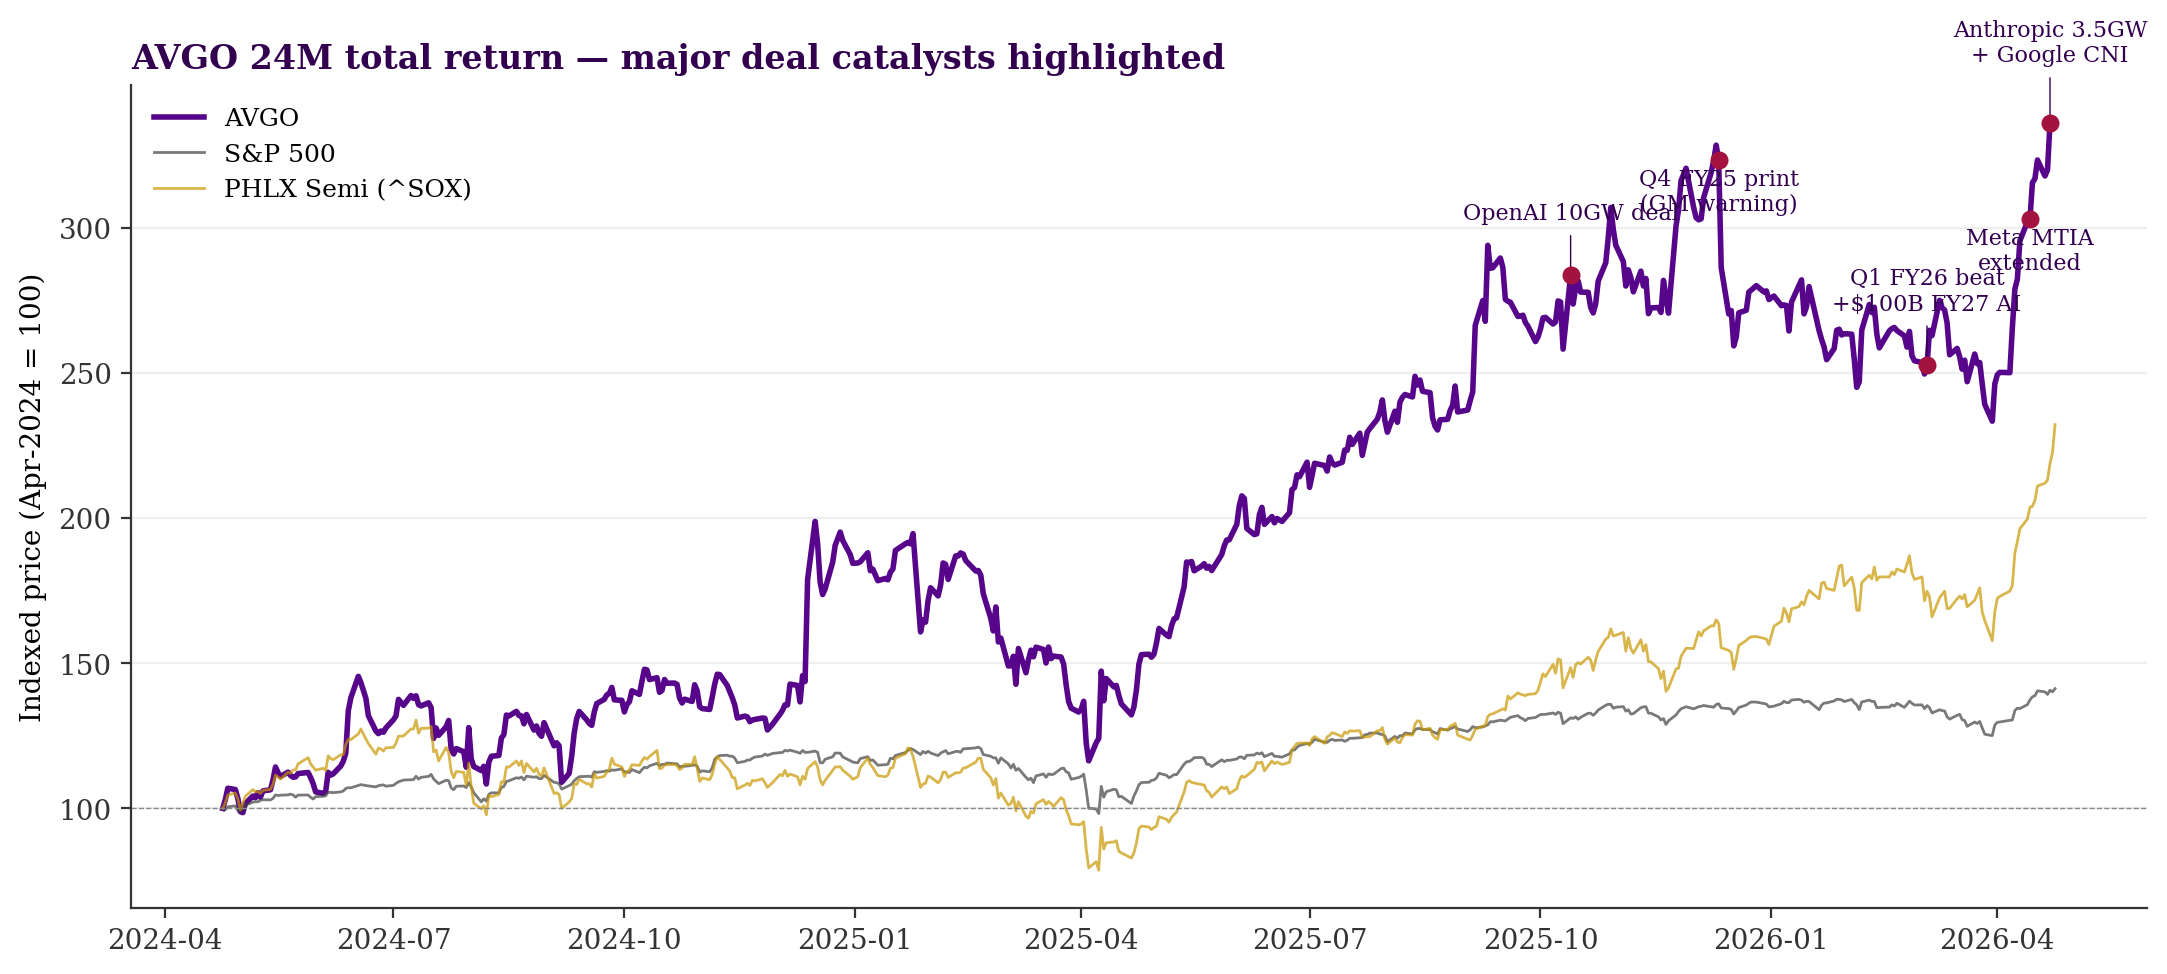
\includegraphics[width=4.4in]{fig1_price_chart.png}};

\node[anchor=north east,inner sep=0pt]
  at ([xshift=-0.55in,yshift=-6.55in]current page.north east) {%
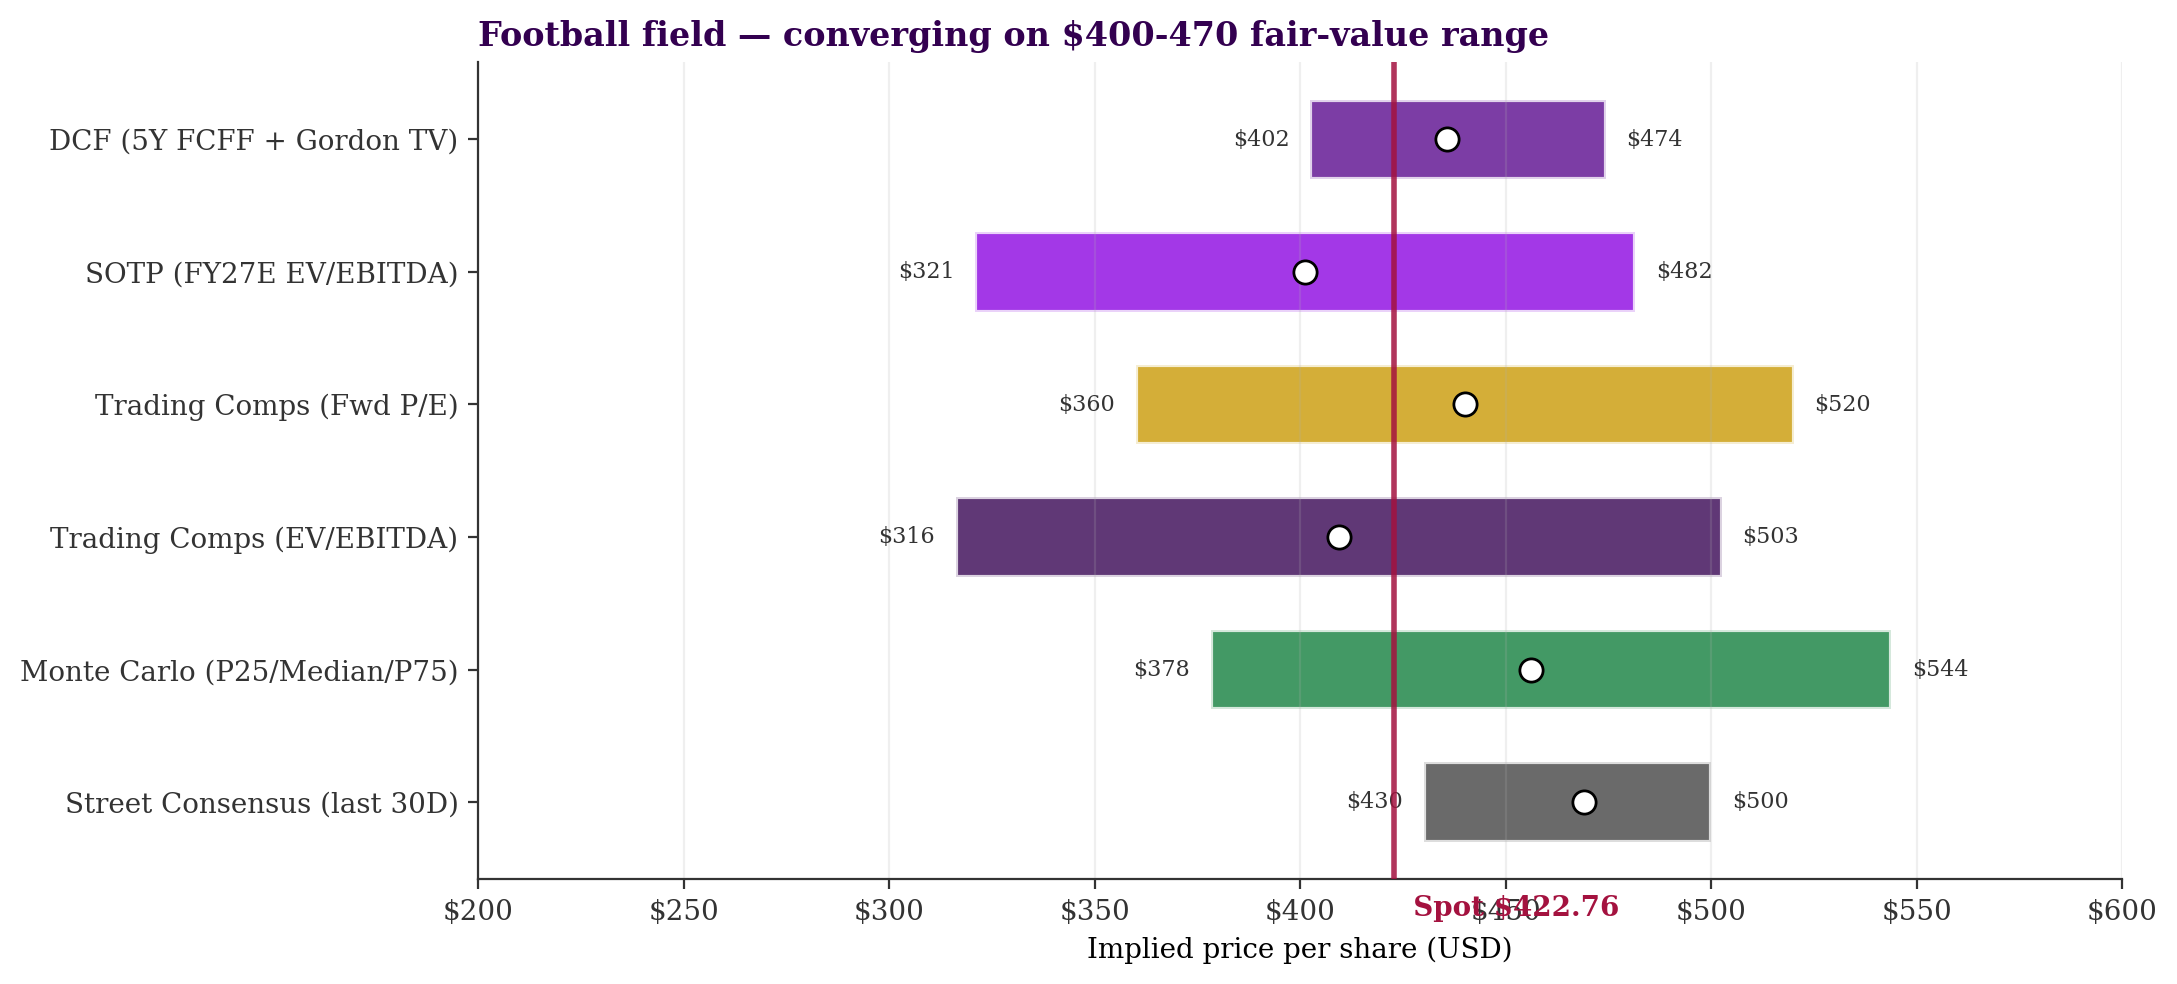
\includegraphics[width=4.4in]{fig4_football_field.png}};

% =============================================================================
% Team photo + byline footer (compact)
% =============================================================================
\node[anchor=south west,inner sep=0pt,text width=7.4in]
  at ([xshift=0.6in,yshift=0.25in]current page.south west) {%
{\color{nyuviolet}\rule{\linewidth}{0.5pt}}\\[-2pt]
{\scriptsize\bfseries\color{nyuviolet}AUTHORS \textbar{} WASHINGTON SQUARE RESEARCH PARTNERS}\\[-3pt]
{\color{nyuviolet}\rule{\linewidth}{0.3pt}}\\[3pt]
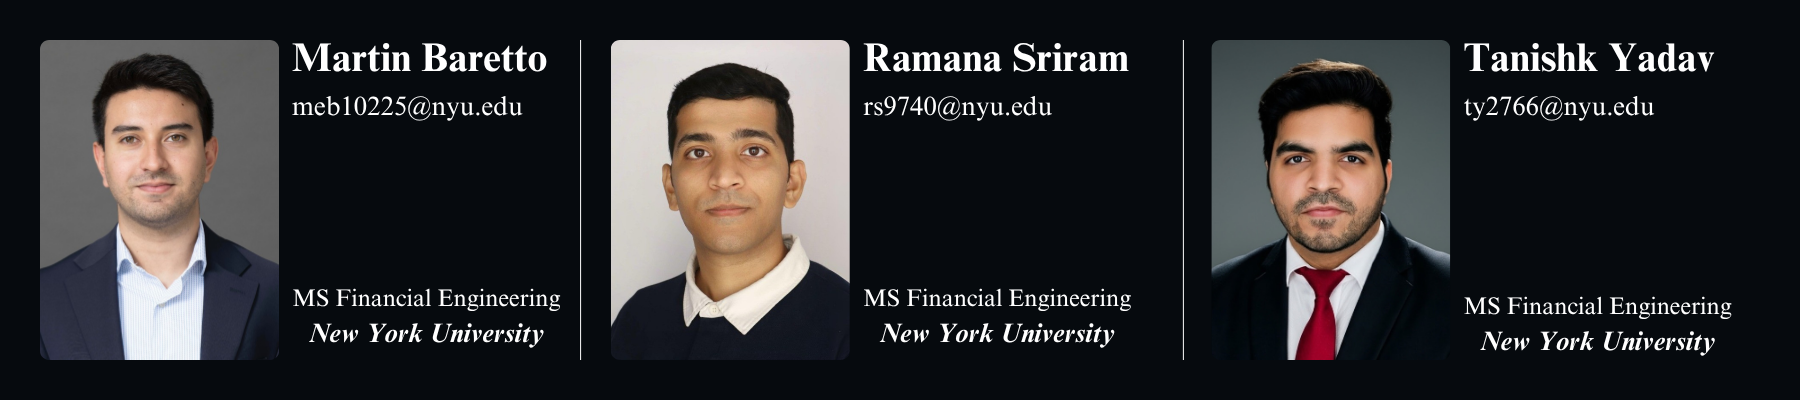
\includegraphics[width=\linewidth,height=1.7in,keepaspectratio]{team_photo.png}\\[1pt]
{\scriptsize\color{nyugrey}\textit{Student-prepared educational research; not investment advice. Data as of 24/25 April 2026.}}
};

\end{tikzpicture}

\restoregeometry
\newpage

% =============================================================================
% INVESTMENT SUMMARY (page 2)
% =============================================================================
\section*{Investment Summary}
\sectionbyline{Lead author: Tanishk Yadav}{Coverage initiation}

\textbf{Recommendation: BUY \textbar{} 12-Month PT: \$475 (12.3\% upside)}

\begin{minipage}[t]{0.55\textwidth}
We initiate coverage of Broadcom (AVGO) with a \textbf{BUY} rating and a December-2026 price target of \$475, representing 12.3\% upside to the 24-April spot price of \$422.76. Our valuation triangulates a \$401--\$474 fair-value range across DCF, sum-of-the-parts, peer comparables, and a 10{,}000-path Monte Carlo simulation that places the median intrinsic price at \$456 with a 60.7\% probability of trading above spot at current levels.

We are constructive on the \textbf{operating story}: AI semiconductor revenue grew 106\% year-over-year in Q1 FY26 to \$8.4 billion, management has line-of-sight to \$100 billion+ in FY27 AI chip revenue across six XPU customers, and the company has secured leading-edge wafer, HBM, and substrate capacity through FY28. Recent deal flow---OpenAI's 10GW co-design partnership (October 2025), Anthropic's 3.5GW commitment via Google Cloud (April 2026), and Meta's MTIA extension through 2029 (April 2026)---pushed Broadcom into the \$2 trillion market-cap club.

We are constructive on \textbf{valuation despite the rally}: shares are up 32.6\% in 30 days but our Monte Carlo's $E[\text{intrinsic}] = \$471$ exceeds spot, and the right tail is fat (P75 \$544, P95 \$711) reflecting realistic upside if FY27 AI revenue prints at the high end of the analyst range (\$130--150B per UBS / Barclays). The 50.8\% probability we calculated under a more conservative \$115B FY27 AI mean rises to 60.7\% at \$125B---closer to the Street midpoint.

Our PT of \$475 sits at the Street median (\$477) and below the mean. We see further upside if the December 2026 FY27 guide validates the \$120B+ AI revenue scale.
\end{minipage}\hfill
\begin{minipage}[t]{0.42\textwidth}
\vspace{0pt}
\begin{tabular}{>{\columncolor{rowshade}}p{3.4cm}p{2.6cm}}
\arrayrulecolor{nyuviolet}\toprule
\multicolumn{2}{c}{\cellcolor{nyuviolet}\color{white}\textbf{Snapshot}}\\
\midrule
Ticker          & AVGO US \\
Sector          & Tech \\
Industry        & Semiconductors \\
CEO             & Hock E. Tan \\
HQ              & Palo Alto, CA \\
Fiscal year-end & 1-Nov \\
Next print      & 5-Jun-26 (Q2) \\
\midrule
\multicolumn{2}{c}{\cellcolor{nyuviolet}\color{white}\textbf{Valuation footprint}}\\
\midrule
DCF (mid)       & \$436 \\
SOTP (mid)      & \$401 \\
Comps P/E (mid) & \$440 \\
Comps EV/EBITDA & \$409 \\
MC median       & \$456 \\
MC P($>$spot)   & 60.7\% \\
Street median   & \$477 \\
\bottomrule
\end{tabular}
\end{minipage}

\subsection*{Five-Point Thesis}

\begin{enumerate}[leftmargin=*,itemsep=4pt]
\item \textbf{The AI thesis is real and the multiple is defensible.} The six-customer XPU portfolio (Google, Meta, ByteDance, SoftBank/ARM, Anthropic via Google, OpenAI) gives Broadcom secular topline growth that few semiconductor peers can match. At 23$\times$ forward P/E, the multiple is in line with the peer median (25.6$\times$).
\item \textbf{Customer concentration is a real risk but a rapidly diversifying one.} Google TPU drives $\sim$50\% of AI revenue today---falling to 35\% by FY27 as Anthropic ($\sim$\$42B), Meta MTIA (multi-GW), and OpenAI (>1GW) ramp. The portfolio effect cushions individual program risk.
\item \textbf{Margins are the upside surprise that has not yet been priced.} Management reversed its prior rack-scale margin warning, now guiding flat 77\% gross margin through FY27 as the mix shifts toward higher-attach networking (40\% of AI revenue in Q2). This alleviates the largest investor overhang from December 2025.
\item \textbf{Competitive moat is wider than market gives credit for.} JPMorgan's primary research suggests Broadcom maintains an 18-month design lead over Google's internal Zebrafish COT effort, and the company has won the next-gen 2nm TPU. Marvell's recent Alphabet engagement is at the early stage and unlikely to displace Broadcom share through 2028.
\item \textbf{Recommendation derived from analysis.} Six valuation methods converge: MC median \$456, DCF \$436, Comps P/E \$440, Comps EV/EBITDA \$409, SOTP \$401, Street median \$477. Our \$475 PT sits at the Street median---a level we view as defensible given the catalyst path through year-end.
\end{enumerate}

\begin{figure}[!ht]
\centering
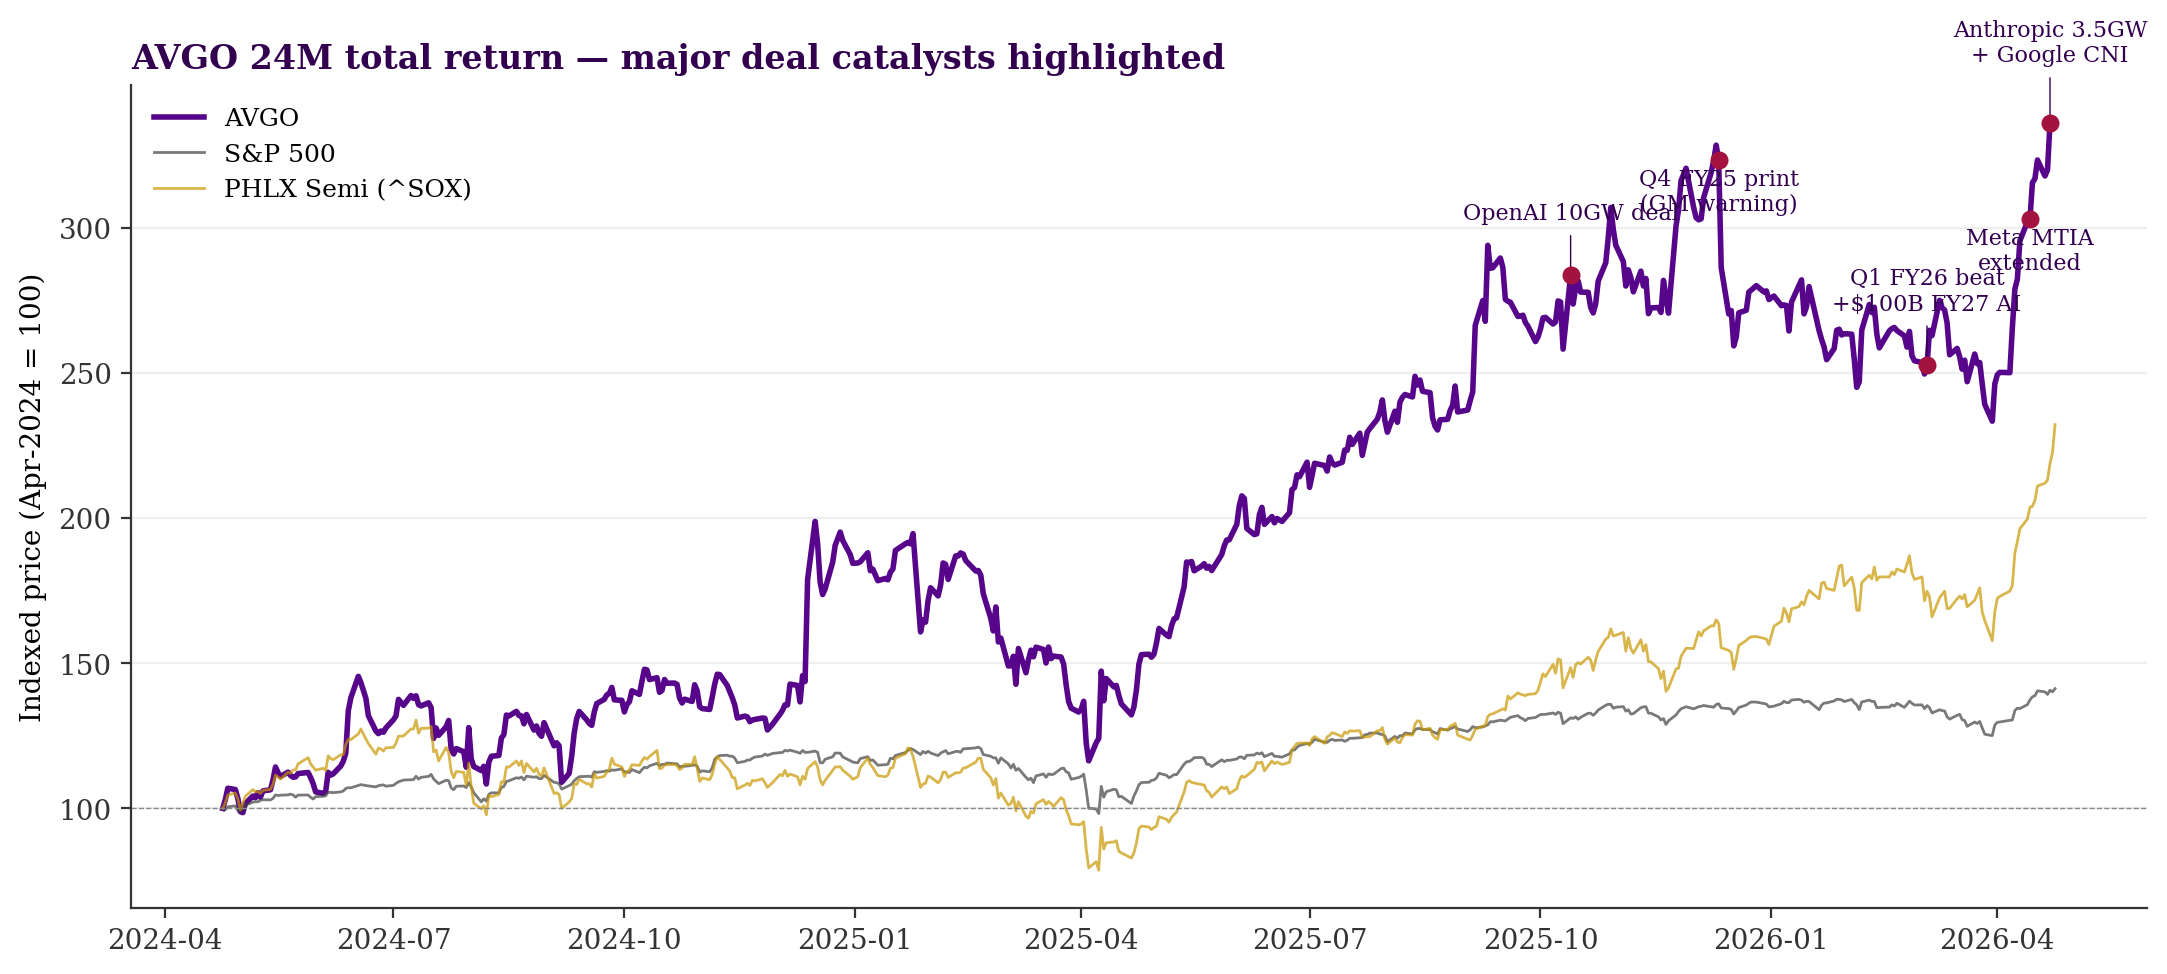
\includegraphics[width=\textwidth]{fig1_price_chart.png}
\caption{AVGO 24-month total return vs.\ S\&P 500 and PHLX Semiconductor Index, with major deal catalysts annotated. Source: Yahoo Finance (yfinance), team analysis.}
\end{figure}

\newpage

% =============================================================================
% BUSINESS DESCRIPTION
% =============================================================================
\section{Business Description}
\sectionbyline{Lead author: Ramana Sriram}{Industry coverage}

Broadcom Inc. designs, manufactures, and sells semiconductors and enterprise infrastructure software through two reporting segments. \textbf{Semiconductor Solutions} (65\% of Q1 FY26 revenue) encompasses custom AI accelerators (XPUs), networking silicon (Tomahawk/Jericho/Trident switching ASICs, SerDes, and optical components), wireless connectivity (FBAR filters, Wi-Fi/Bluetooth combos for the iPhone), broadband (cable/fiber gateways), storage (Fibre Channel HBAs, RAID), and industrial connectivity. \textbf{Infrastructure Software} (35\%) was rebuilt through the \$69 billion VMware acquisition in November 2023 and now combines VMware Cloud Foundation, Symantec enterprise security, and the legacy CA mainframe business.

The company was created by the 2016 reverse merger of Avago Technologies and the original Broadcom Corporation. Under CEO Hock Tan---now in his twentieth year leading the combined entity---Broadcom has executed a serial M\&A playbook: Brocade (2017), CA (2018), Symantec Enterprise (2019), and VMware (2023). The model strips overhead and re-prices subscriptions toward the largest enterprise customers. Five-year revenue CAGR is 23.5\%; non-GAAP operating margin expanded from 47\% in FY20 to 66.4\% in Q1 FY26.

\subsection{Segment economics}

\begin{table}[!ht]
\centering
\small
\rowcolors{2}{rowshade}{white}
\begin{tabular}{p{4.6cm}p{3.0cm}p{3.5cm}p{3.5cm}}
\arrayrulecolor{nyuviolet}\toprule
\rowcolor{nyuviolet}\color{white}\textbf{Segment} & \color{white}\textbf{FY25 revenue} & \color{white}\textbf{Gross margin} & \color{white}\textbf{Demand driver} \\
\midrule
AI Semiconductor (XPU + networking) & \$24.5B (38\%)  & $\sim$60--65\% & Hyperscaler capex \\
Non-AI Semiconductor               & \$15.5B (24\%)  & $\sim$70--72\% & End-market cyclical \\
Infrastructure Software            & \$23.9B (37\%)  & $\sim$92--93\% & Enterprise refresh + VCF migration \\
\arrayrulecolor{nyuviolet}\bottomrule
\end{tabular}
\caption{FY25 segment composition. Source: Broadcom Q4 FY25 8-K, Mizuho 4-Mar-26.}
\end{table}

\subsection{The XPU customer roster}

Management discloses that Broadcom now serves six committed XPU (custom accelerator) customers. JPMorgan and Mizuho identify them through a process of elimination as: Google (TPU, the anchor program since 2014), Meta (MTIA), ByteDance, an ARM/SoftBank-linked program (likely Stargate), Anthropic (via the Google three-way), and OpenAI (the October 2025 deal). The six-customer base, plus continued networking attach, supports management's ``more than \$100 billion'' FY27 AI revenue line-of-sight statement on the Q1 FY26 earnings call.

\begin{figure}[!ht]
\centering
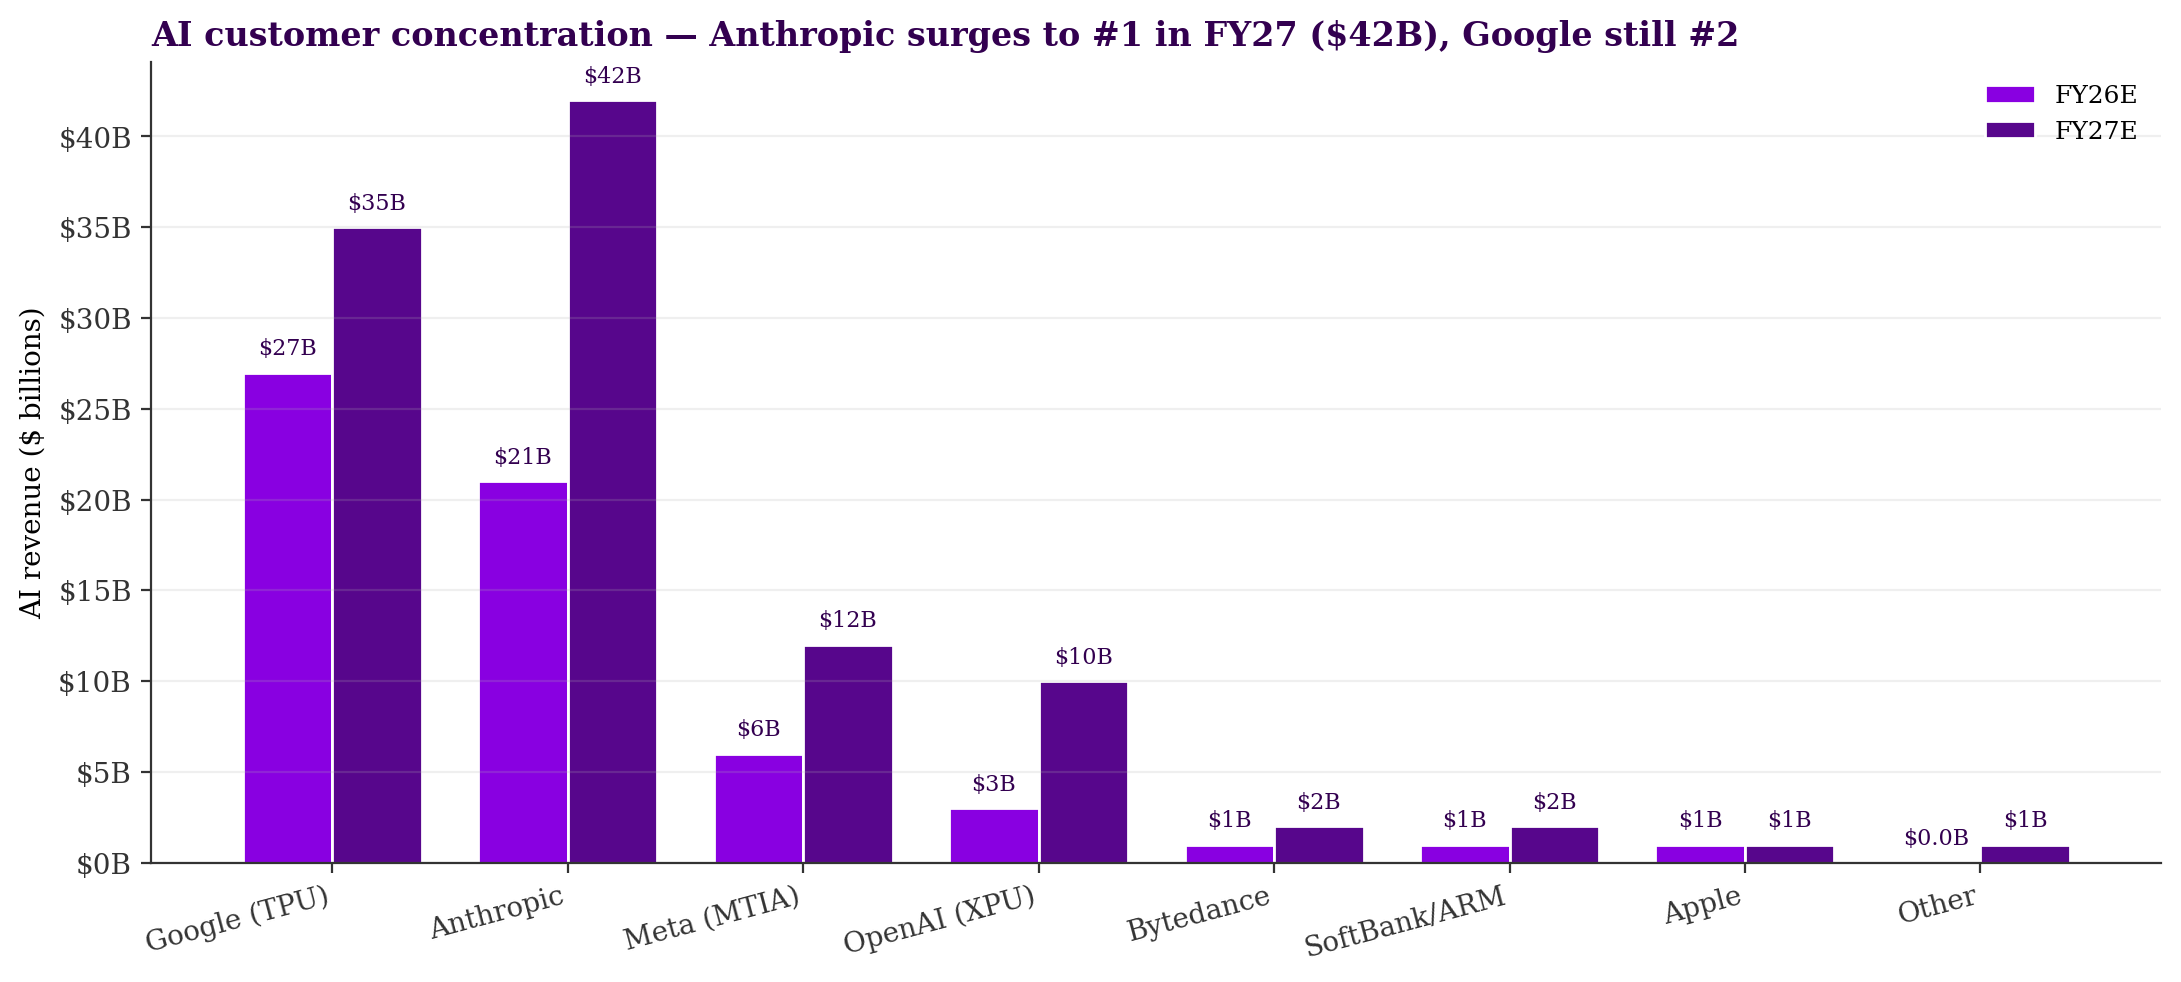
\includegraphics[width=0.96\textwidth]{fig8_ai_customers.png}
\caption{Customer-level AI revenue breakdown, FY26E vs.\ FY27E. Anthropic surges to the top spot in FY27 on the 3GW TPU rack ramp. Source: Mizuho Exhibit 1 (4-Mar-26), JPMorgan (5-Mar-26), team estimates.}
\end{figure}

\newpage

% =============================================================================
% RECENT DEALS
% =============================================================================
\section{Recent Strategic Catalysts}
\sectionbyline{Lead author: Ramana Sriram}{Industry coverage}

The four months between Q1 FY26 earnings (4-Mar-26) and the date of this report contain the most consequential dealflow in Broadcom's history outside of the VMware close.

\subsection{OpenAI: 10 GW custom XPU partnership (October 2025)}
OpenAI and Broadcom signed a co-development agreement under which OpenAI designs the accelerator while Broadcom owns the manufacturing, networking, and system integration. Total deployment of 10 gigawatts spans late 2026 through end-2029. Mizuho's Vijay Rakesh estimates this is the program now identified as ``Customer 6'' in Broadcom disclosures and embeds \$3 billion of FY26 revenue and \$10 billion in FY27.

\subsection{Anthropic: 3.5 GW three-way deal (April 2026)}
Announced jointly by Anthropic, Google Cloud, and Broadcom, this commitment routes Anthropic's compute through Google Cloud running on Broadcom-fabricated TPU silicon. Mizuho models \$21 billion of recognized AI revenue at Broadcom in 2026 stepping to \$42 billion in 2027, making Anthropic the single largest contributor to Broadcom's FY27 AI mix---surpassing internal Google demand.

\subsection{Meta MTIA extension through 2029 (April 2026)}
Meta's custom inference chip program (MTIA, internally codenamed Athena/Iris/Olympus) was extended for multi-gigawatt deployments through 2029. Wells Fargo models the Meta program at multiple gigawatts by FY27 with a clear vector to expand vertically integrated AI infrastructure away from Nvidia GPU dependence.

\subsection{Google TPU ``Sunfish'' 3nm ramp + Cloud Network Insights (April 2026)}
Beyond chips, Broadcom announced an expanded software collaboration with Google Cloud on 22 April 2026 to launch Cloud Network Insights for multi-cloud network observability. While modest financially, it signals strategic depth in the Broadcom-Google relationship beyond hardware.

\begin{figure}[!ht]
\centering
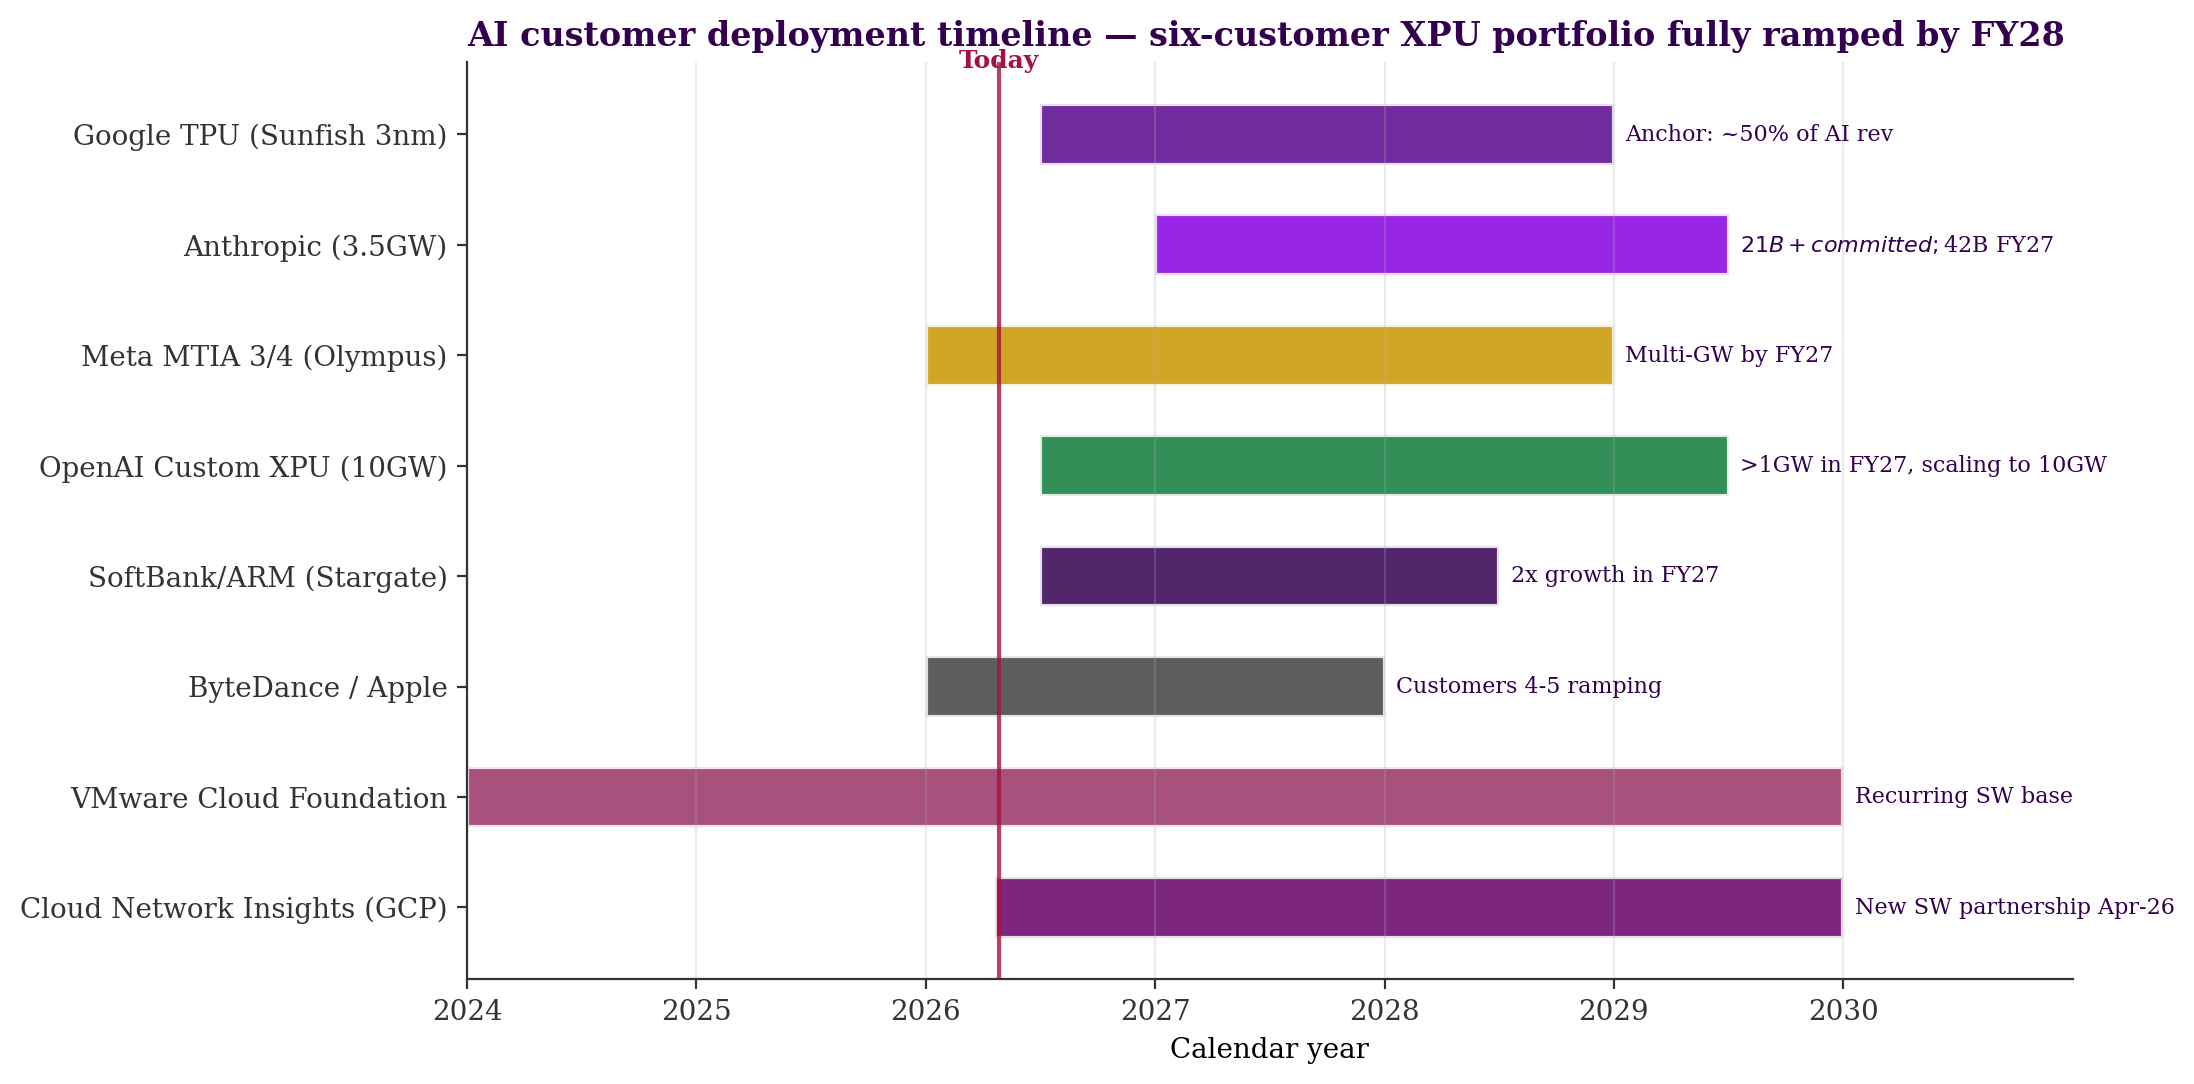
\includegraphics[width=\textwidth]{fig9_deal_timeline.png}
\caption{AI customer deployment timeline. Six-customer XPU portfolio fully ramped by FY28. Source: Company disclosures, JPMorgan, UBS, Mizuho team analysis.}
\end{figure}

\subsection{Sell-side reaction}

Eleven sell-side firms updated their models post Q1 FY26. The Street is clearly bullish, but the dispersion is wide. The condensed positioning snapshot is shown below, followed by a more detailed breakdown:

\begin{table}[!ht]
\centering
\small
\rowcolors{2}{rowshade}{white}
\begin{tabular}{p{2.8cm}lp{1.4cm}p{1.4cm}}
\arrayrulecolor{nyuviolet}\toprule
\rowcolor{nyuviolet}\color{white}\textbf{Firm} & \color{white}\textbf{Rating} & \color{white}\textbf{PT (\$)} & \color{white}\textbf{CY27 EPS} \\
\midrule
JPMorgan      & OW  & 500 & 20.45 \\
Barclays      & OW  & 500 & 18.60 \\
Mizuho        & OP  & 480 & 18.30 \\
UBS           & B   & 475 & 22.76 \\
Wells Fargo   & OW  & 430 & 20.24 \\
Deutsche Bank & B   & 430 & --    \\
Evercore ISI  & OP  & 582 & --    \\
Citi          & B   & 460 & --    \\
BofA          & B   & 445 & --    \\
\arrayrulecolor{nyuviolet}\midrule
\textbf{Median (n=11)} & \textbf{8 OW} & \textbf{477} & -- \\
\arrayrulecolor{nyuviolet}\bottomrule
\end{tabular}
\caption{Street positioning summary. Source: Sell-side reports (Mar--Apr 2026); team analysis.}
\end{table}

\begin{table}[!ht]
\centering
\small
\rowcolors{2}{rowshade}{white}
\begin{tabular}{p{3.4cm}p{2.0cm}p{1.6cm}p{2.2cm}p{1.8cm}p{3.4cm}}
\arrayrulecolor{nyuviolet}\toprule
\rowcolor{nyuviolet}\color{white}\textbf{Firm} & \color{white}\textbf{Analyst} & \color{white}\textbf{Rating} & \color{white}\textbf{PT (\$)} & \color{white}\textbf{CY27 EPS} & \color{white}\textbf{Target multiple} \\
\midrule
JPMorgan      & H.\ Sur     & OW & 500 & 20.45 & 23--25$\times$ \\
Barclays      & T.\ O'Malley & OW & 500 & 18.60 & 27$\times$ \\
Mizuho        & V.\ Rakesh   & OP & 480 & 18.30 & 26$\times$ \\
UBS           & T.\ Arcuri   & B  & 475 & 22.76 & 21$\times$ \\
Wells Fargo   & A.\ Rakers   & OW & 430 & 20.24 & 21$\times$ \\
Deutsche Bank & R.\ Seymore  & B  & 430 & --    & 23$\times$ \\
\arrayrulecolor{nyuviolet}\bottomrule
\end{tabular}
\caption{Major sell-side post-Q1 FY26 updates. Source: Sell-side reports (Mar 2026); team analysis.}
\end{table}

The mean PT of the eleven covering firms in our dataset is \$469; the median is \$477. Eight of eleven sit above the current spot price.

\begin{figure}[!ht]
\centering
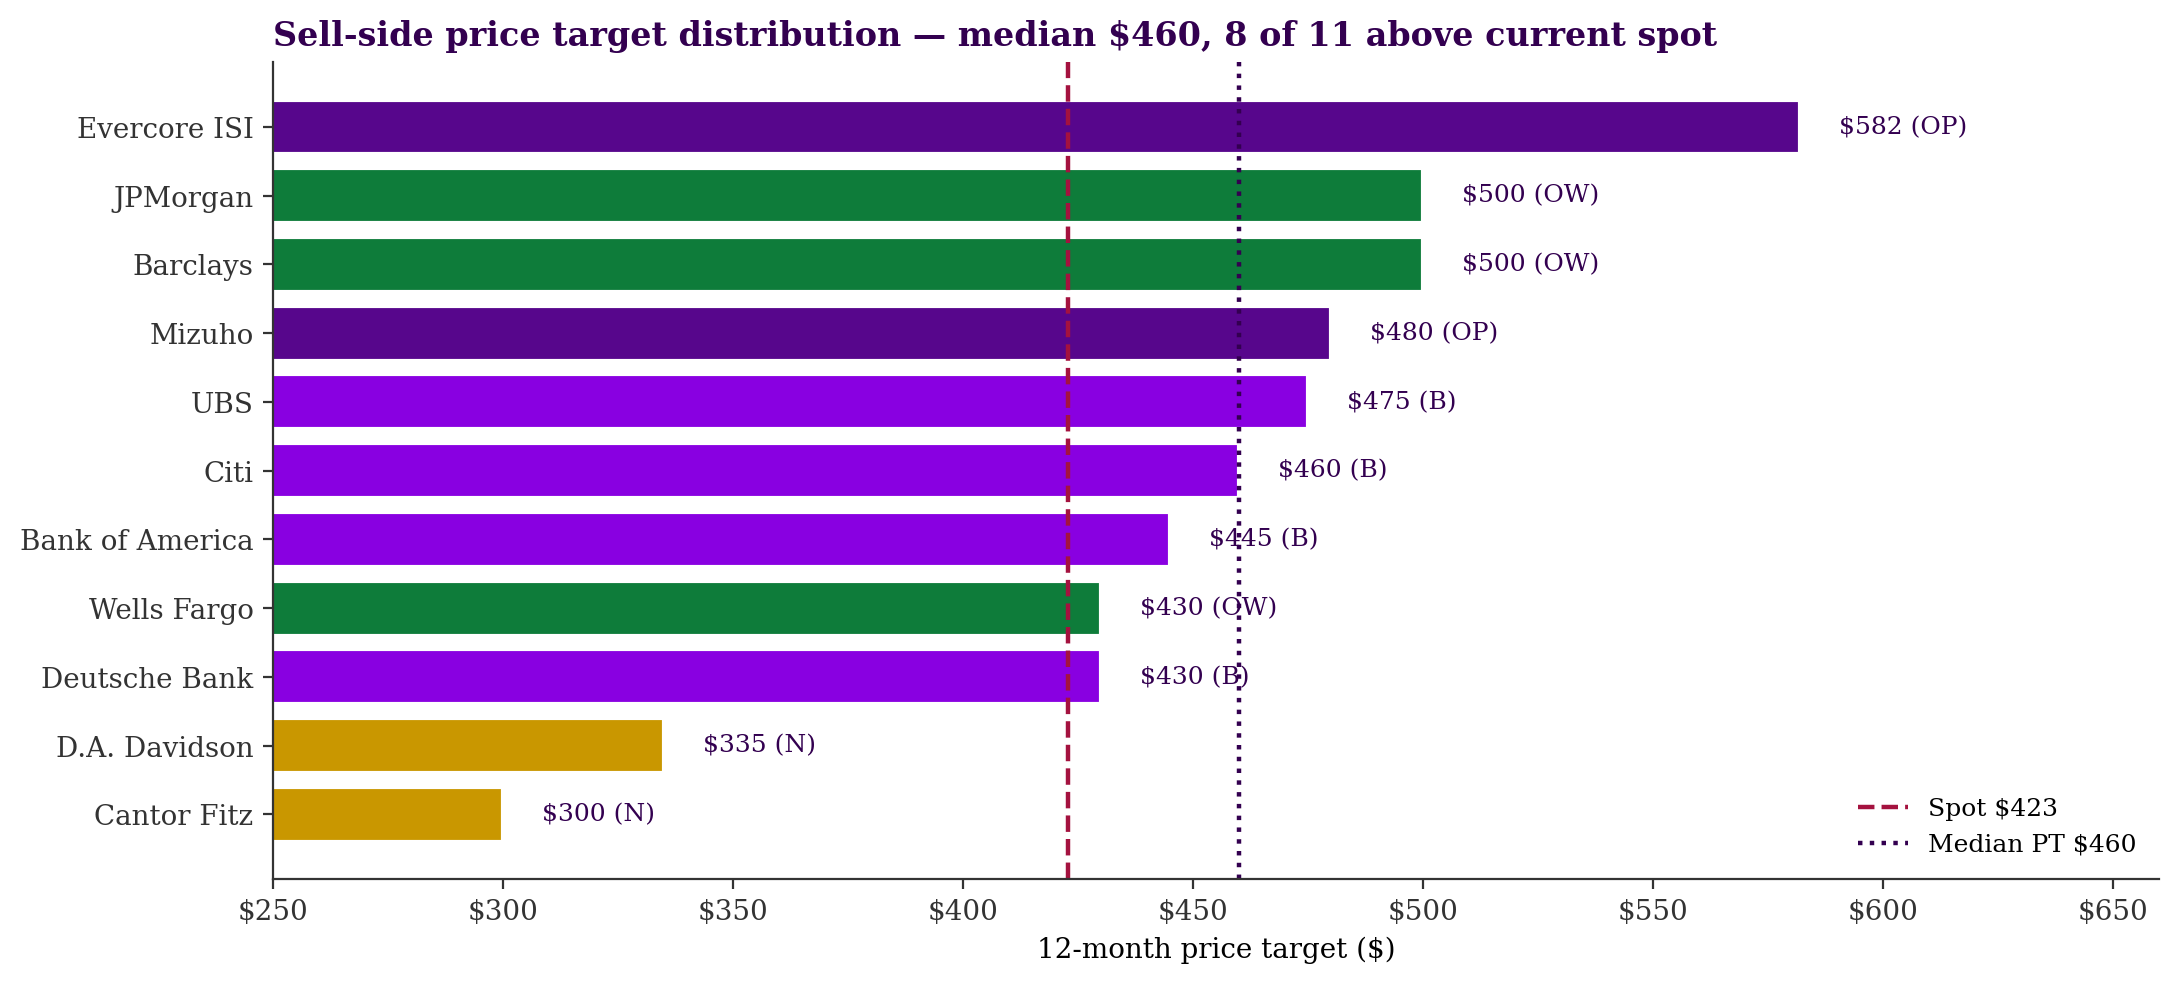
\includegraphics[width=\textwidth]{fig12_analyst_pts.png}
\caption{Sell-side price-target distribution. Median \$477; 8 of 11 firms above spot. Source: Benzinga, individual broker reports.}
\end{figure}

\newpage

% =============================================================================
% FINANCIAL ANALYSIS
% =============================================================================
\section{Financial Analysis}
\sectionbyline{Lead author: Tanishk Yadav}{Modeling \& projections}

\subsection{Q1 FY26 results recap}

Broadcom delivered a clean beat-and-raise quarter on 4 March 2026:

\begin{itemize}[leftmargin=*]
\item \textbf{Revenue:} \$19.31 billion (+29.5\% YoY) vs.\ Street \$19.26 billion. AI semiconductor revenue \$8.4 billion (+106\% YoY); non-AI semi \$4.1 billion; software \$6.8 billion.
\item \textbf{Margins:} Gross margin 77.0\%, EBITDA margin 68\%, operating margin 66.4\%.
\item \textbf{EPS:} \$2.05 non-GAAP (+28\% YoY) vs.\ Street \$2.03.
\item \textbf{Cash flow:} \$8.0 billion of free cash flow (41\% of revenue); ended quarter with \$14.2 billion of cash and \$51 billion of net debt; \$10 billion incremental authorization to the buyback program.
\item \textbf{Q2 FY26 guide:} Revenue \$22.0 billion (+47\% YoY), AI revenue \$10.7 billion (+139\% YoY), gross margin flat 77\%.
\end{itemize}

The single most consequential commentary was the reversal of the December 2025 margin warning: management now expects gross margin to remain in the high-70s through the Anthropic rack-scale ramp, citing a higher-attach networking mix and pricing concessions on rack components. JPMorgan, UBS, and Mizuho all flagged this as the key positive surprise.

\subsection{Five-year operating projection}

We project FY26E revenue of \$105 billion (+64\% YoY) and FY30E revenue of \$292 billion, with AI semi growing from \$60 billion in FY26 to \$235 billion by FY30 (a 41\% five-year CAGR). Our FY27 AI revenue assumption of \$115 billion sits at the midpoint of the analyst range (\$100--150 billion) and within management's stated ``more than \$100 billion'' guidance.

\begin{figure}[!ht]
\centering
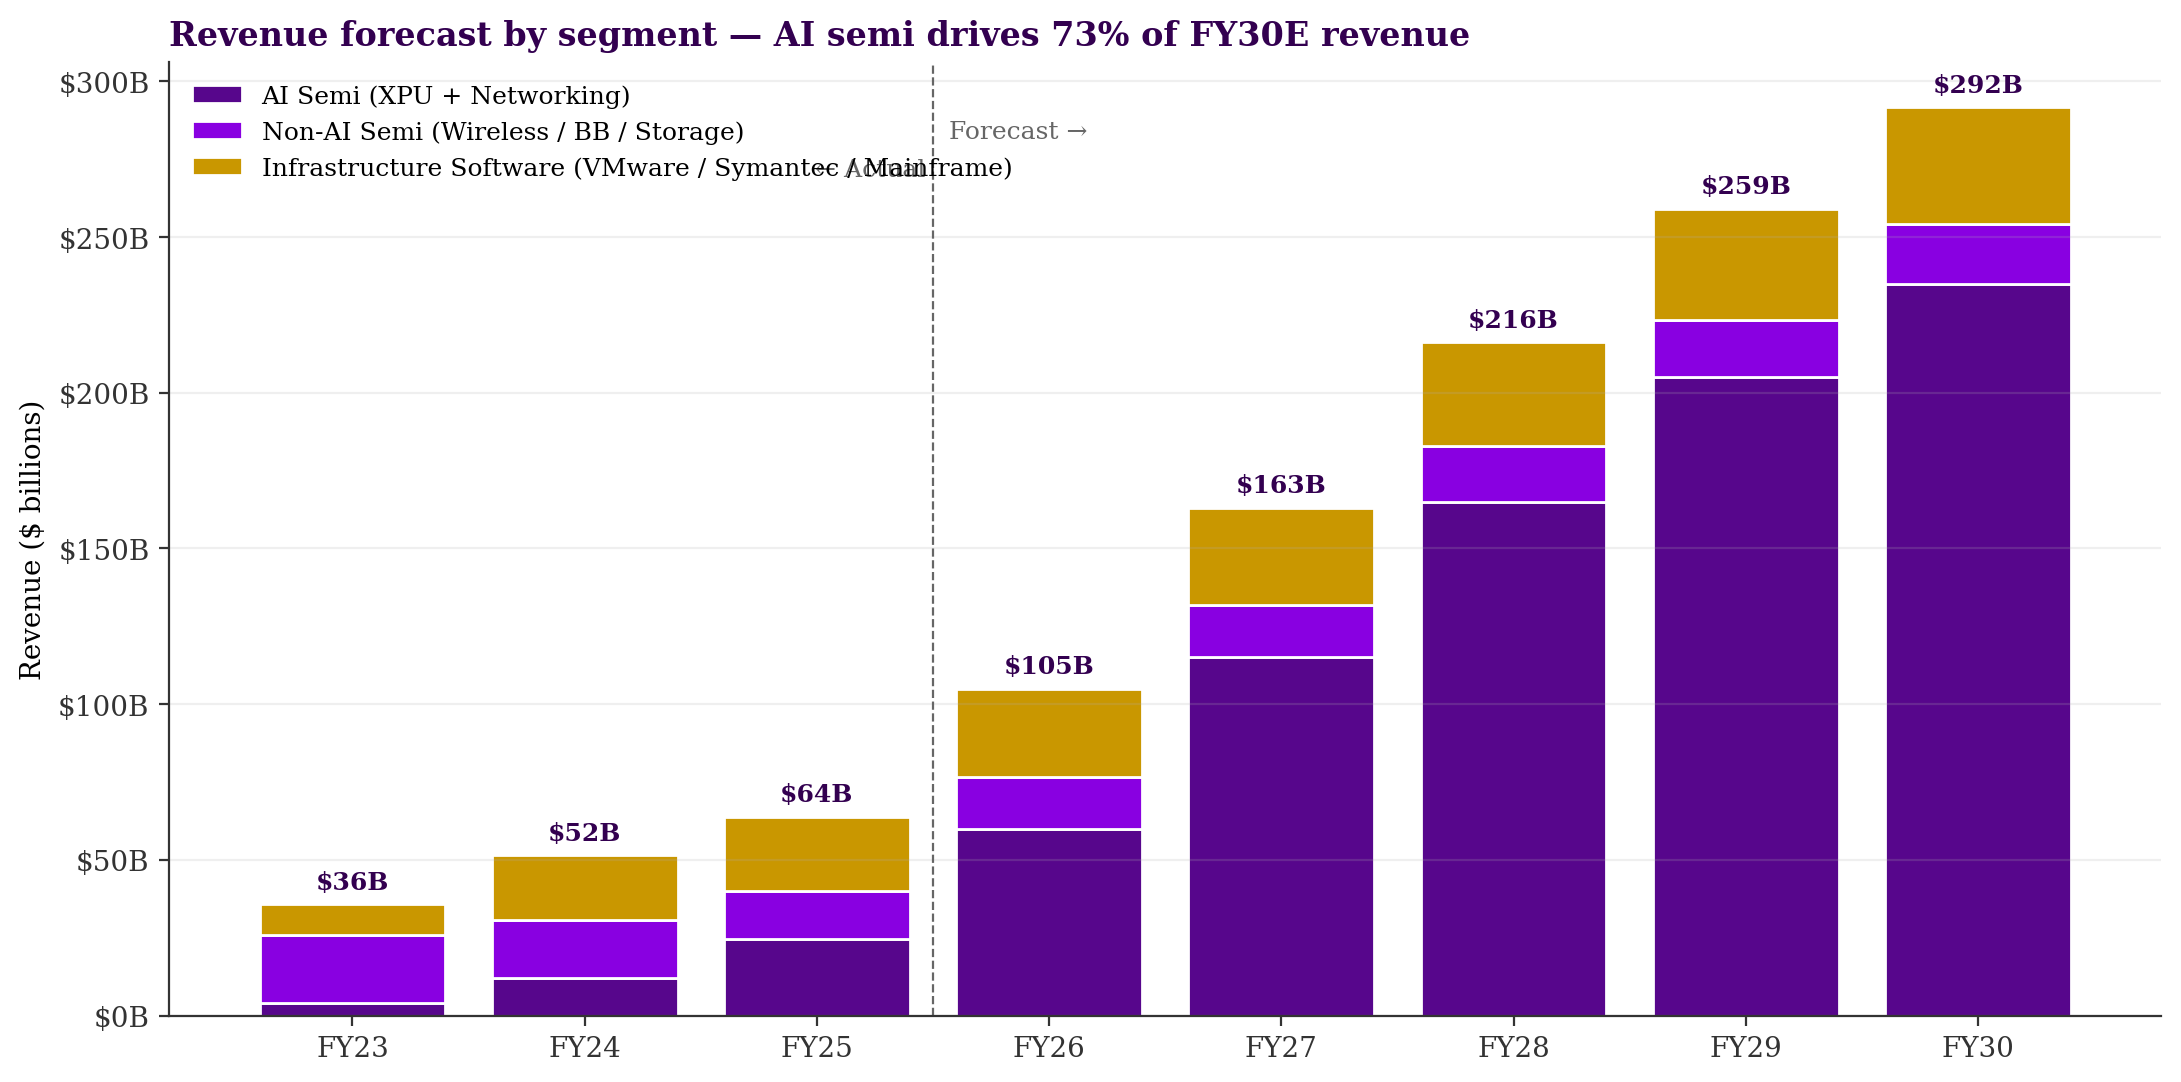
\includegraphics[width=\textwidth]{fig2_revenue_bridge.png}
\caption{Revenue forecast by segment, FY23A--FY30E. AI semi reaches 73\% of total revenue by FY30. Source: Company filings, team estimates.}
\end{figure}

\begin{table}[!ht]
\centering
\small
\rowcolors{2}{rowshade}{white}
\setlength{\tabcolsep}{4pt}
\begin{tabular}{p{4.0cm}rrrrrrr}
\arrayrulecolor{nyuviolet}\toprule
\rowcolor{nyuviolet}\color{white}\textbf{(\$ in millions)} & \color{white}\textbf{FY24A} & \color{white}\textbf{FY25A} & \color{white}\textbf{FY26E} & \color{white}\textbf{FY27E} & \color{white}\textbf{FY28E} & \color{white}\textbf{FY29E} & \color{white}\textbf{FY30E} \\
\midrule
AI Semiconductor             & 12{,}200 & 24{,}500 & 60{,}000 & 115{,}000 & 165{,}000 & 205{,}000 & 235{,}000 \\
Non-AI Semiconductor          & 18{,}500 & 15{,}500 & 16{,}500 & 17{,}000  & 17{,}750  & 18{,}500  & 19{,}250  \\
Infrastructure Software       & 20{,}800 & 23{,}900 & 28{,}500 & 31{,}000  & 33{,}500  & 35{,}500  & 37{,}500  \\
\midrule
\textbf{Total Revenue}        & \textbf{51{,}500} & \textbf{63{,}900} & \textbf{105{,}000} & \textbf{163{,}000} & \textbf{216{,}250} & \textbf{259{,}000} & \textbf{291{,}750} \\
\textbf{YoY growth}           & --       & 24.0\%   & 64.4\%   & 55.2\%   & 32.7\%   & 19.8\%   & 12.6\%   \\
\midrule
Gross margin                  & 62.6\%   & 74.5\%   & 77.0\%   & 77.5\%   & 78.0\%   & 78.0\%   & 78.0\%   \\
EBITDA                        & 31{,}900 & 43{,}200 & 73{,}200 & 115{,}700 & 155{,}100 & 186{,}200 & 209{,}800 \\
EBITDA margin                 & 61.9\%   & 67.7\%   & 69.7\%   & 71.0\%   & 71.7\%   & 71.9\%   & 71.9\%   \\
FCFF                          & 21{,}600 & 26{,}900 & 57{,}900 & 91{,}600 & 123{,}200 & 148{,}500 & 167{,}200 \\
\arrayrulecolor{nyuviolet}\bottomrule
\end{tabular}
\caption{Operating projection. Source: Company 10-K, Q1 FY26 8-K (5-Mar-26), team estimates.}
\end{table}

\begin{figure}[!ht]
\centering
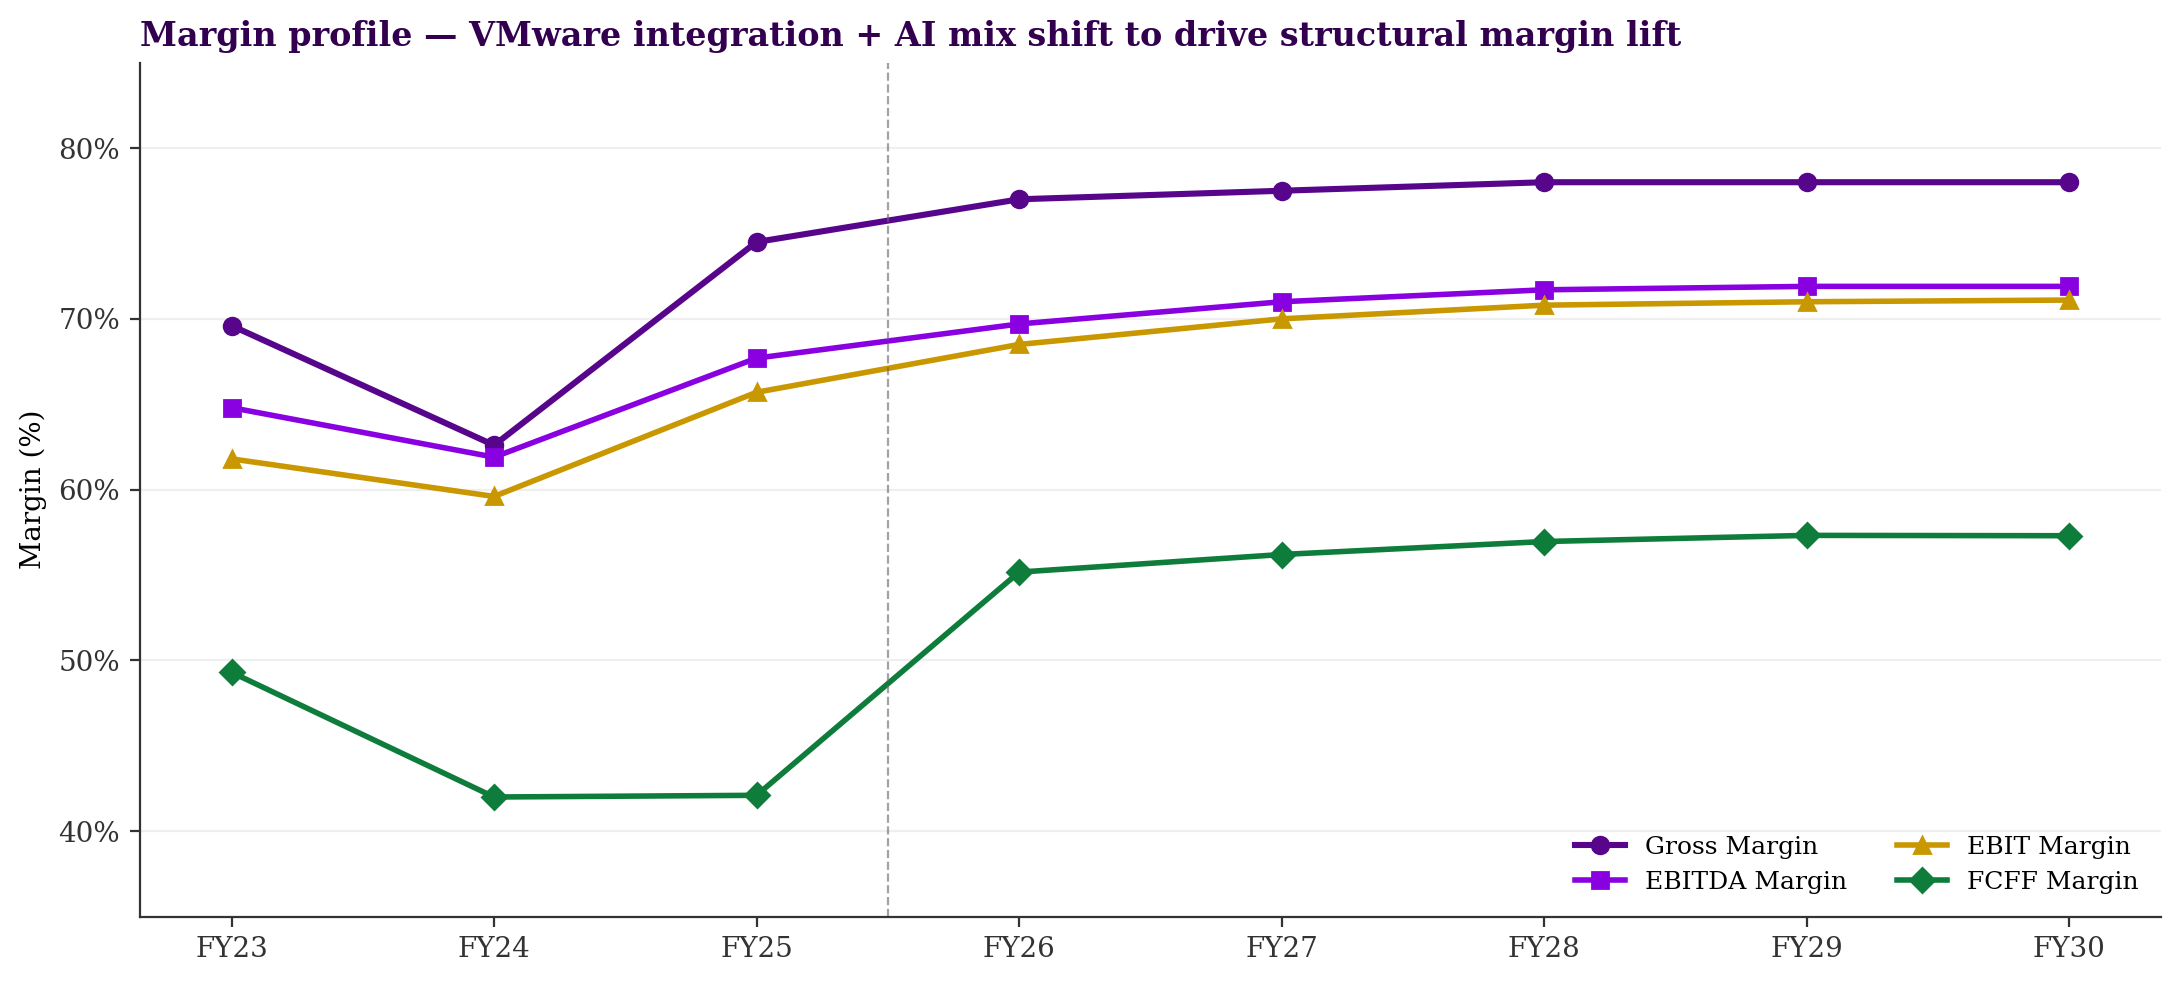
\includegraphics[width=\textwidth]{fig3_margins.png}
\caption{Margin profile, historical and projected. Source: Company filings, team analysis.}
\end{figure}

\newpage

% =============================================================================
% VALUATION
% =============================================================================
\section{Valuation}
\sectionbyline{Lead author: Martin Baretto}{Valuation lead}

We employ four discrete methods and synthesize them in a football-field framework.

\subsection{DCF analysis}

\textbf{WACC build.} We use a 9.4\% weighted-average cost of capital, derived from a 4.31\% risk-free rate (10-year U.S. Treasury, 24-Apr-26), a 5.0\% equity risk premium, and a 1.20 levered beta (Bloomberg two-year weekly, consistent with sell-side convention). The 5-year daily beta of 1.633 reflects elevated AI-cycle volatility and is reported separately; we test both in our sensitivity analysis. Pre-tax cost of debt of 5.0\% (AVGO senior notes blended yield), 18\% effective tax rate, and a 15\% target debt weight yield WACC of 9.38\%.

\textbf{Forecast horizon.} Five-year explicit forecast of FCFF (FY26E--FY30E), with mid-year discounting, plus a Gordon-growth terminal value at 3.0\% perpetuity growth. Terminal value represents 80\% of total enterprise value---a high but not unreasonable share for a growth franchise.

\textbf{Result.} The base-case DCF implies a price of \$444 per share (5.1\% upside), with the WACC$\times$g sensitivity producing a \$402--\$474 range at $\pm$100bps WACC and base terminal growth.

\begin{figure}[!ht]
\centering
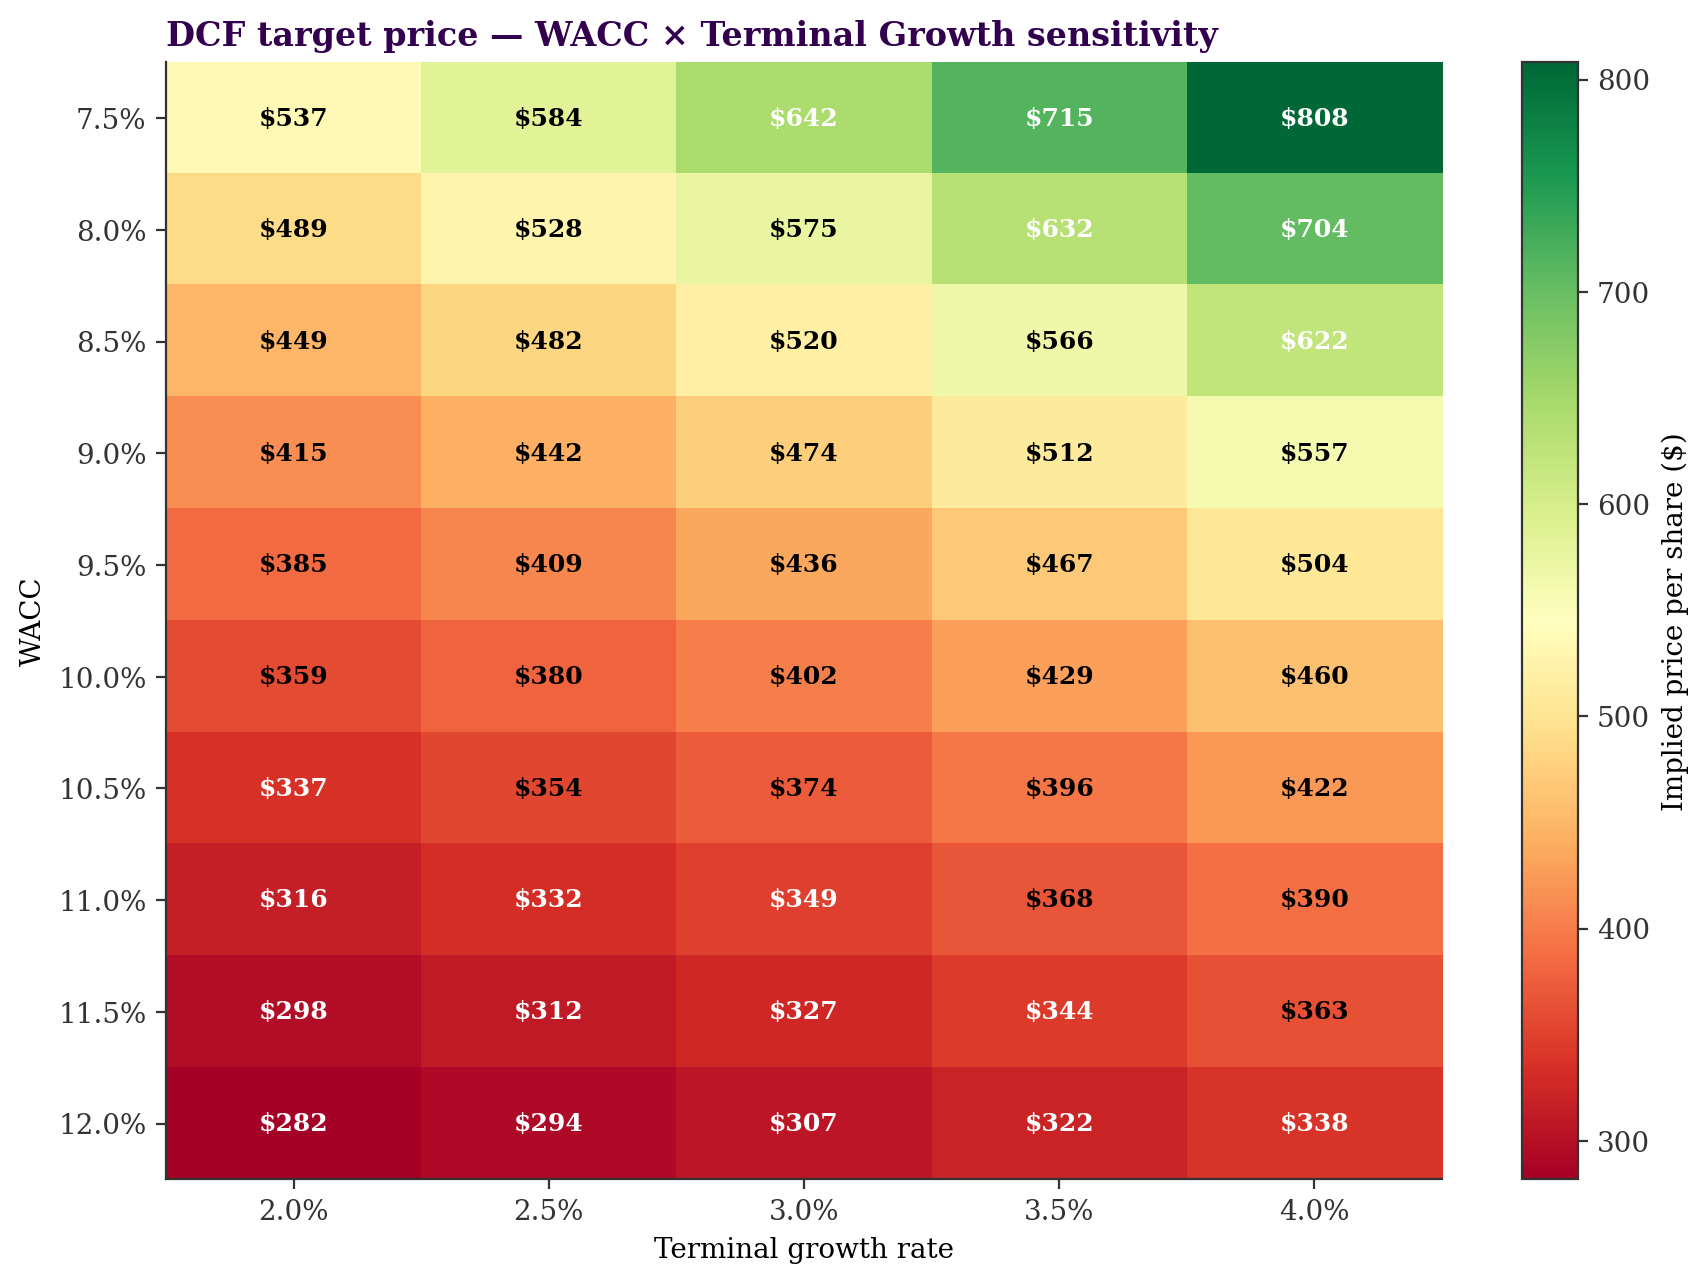
\includegraphics[width=0.92\textwidth]{fig6_sensitivity.png}
\caption{DCF sensitivity: implied price by WACC and terminal growth rate. Source: Team analysis.}
\end{figure}

\begin{figure}[!ht]
\centering
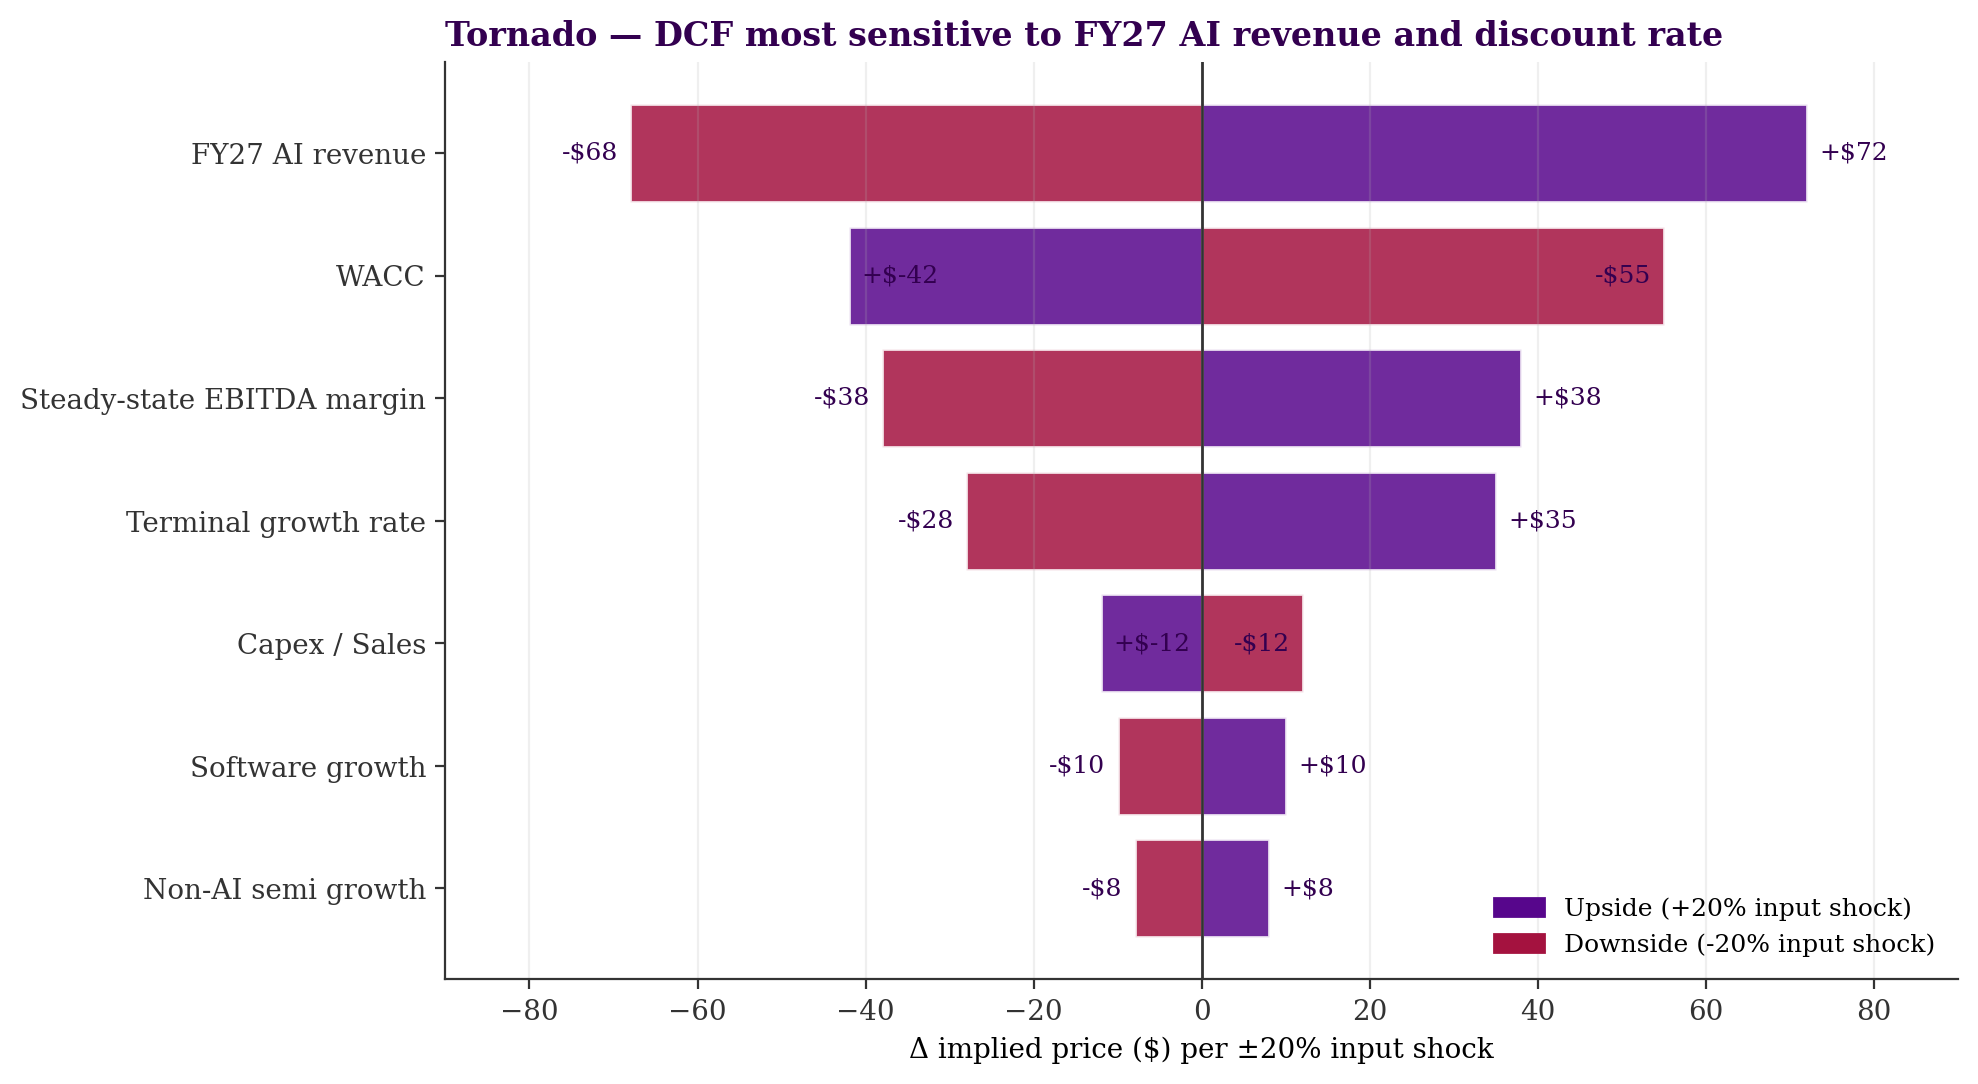
\includegraphics[width=\textwidth]{fig10_tornado.png}
\caption{Tornado chart: DCF most sensitive to FY27 AI revenue and WACC. Source: Team analysis.}
\end{figure}

\subsection{Sum-of-the-parts}

We split Broadcom into its two reporting segments and apply segment-pure peer multiples to FY27E EBITDA:

\begin{table}[!ht]
\centering
\small
\rowcolors{2}{rowshade}{white}
\setlength{\tabcolsep}{4pt}
\begin{tabular}{p{4.6cm}rrrrrr}
\arrayrulecolor{nyuviolet}\toprule
\rowcolor{nyuviolet}\color{white}\textbf{Segment} & \color{white}\textbf{FY27E Rev} & \color{white}\textbf{EBITDA \%} & \color{white}\textbf{EBITDA} & \color{white}\textbf{Mult Low} & \color{white}\textbf{Mid} & \color{white}\textbf{High} \\
\midrule
Semi Solutions          & 132{,}000 & 62.0\% & 81{,}840 & 16.0$\times$ & 20.0$\times$ & 24.0$\times$ \\
Infrastructure Software & 31{,}000  & 77.0\% & 23{,}870 & 14.0$\times$ & 17.0$\times$ & 20.0$\times$ \\
\midrule
\multicolumn{4}{r}{\textbf{Total EV (\$mn)}}              & 1{,}643{,}620 & 2{,}042{,}590 & 2{,}441{,}560 \\
\multicolumn{4}{r}{Less net debt}                          & 48{,}958      & 48{,}958      & 48{,}958      \\
\multicolumn{4}{r}{\textbf{Implied price per share (\$)}}  & \textbf{321}  & \textbf{401}  & \textbf{482}  \\
\arrayrulecolor{nyuviolet}\bottomrule
\end{tabular}
\caption{SOTP valuation, FY27E. Source: Team analysis.}
\end{table}

\subsection{Trading comparables}

We benchmark Broadcom against seven semiconductor peers (NVDA, AMD, MRVL, QCOM, TXN, INTC, TSM). Peer median forward P/E is 25.6$\times$; median EV/EBITDA is 33.9$\times$ TTM (skewed by AMD/MRVL). Applying conservative multiples to our \$20.00 CY27E EPS estimate (vs.\ analyst mean of \$19.85):

\begin{table}[!ht]
\centering
\small
\begin{tabular}{p{4.5cm}p{2.5cm}p{2.5cm}p{2.5cm}}
\arrayrulecolor{nyuviolet}\toprule
\rowcolor{nyuviolet}\color{white}\textbf{Multiple} & \color{white}\textbf{Low} & \color{white}\textbf{Mid} & \color{white}\textbf{High} \\
\midrule
Forward P/E (on CY27E EPS \$20.00)        & 18$\times$ \$360  & 22$\times$ \$440 & 26$\times$ \$520 \\
EV/EBITDA (on FY27E EBITDA \$115.7B)      & 14$\times$ \$316  & 18$\times$ \$409 & 22$\times$ \$503 \\
\arrayrulecolor{nyuviolet}\bottomrule
\end{tabular}
\caption{Trading comps implied price ranges. Source: yfinance peer data, team analysis.}
\end{table}

\begin{figure}[!ht]
\centering
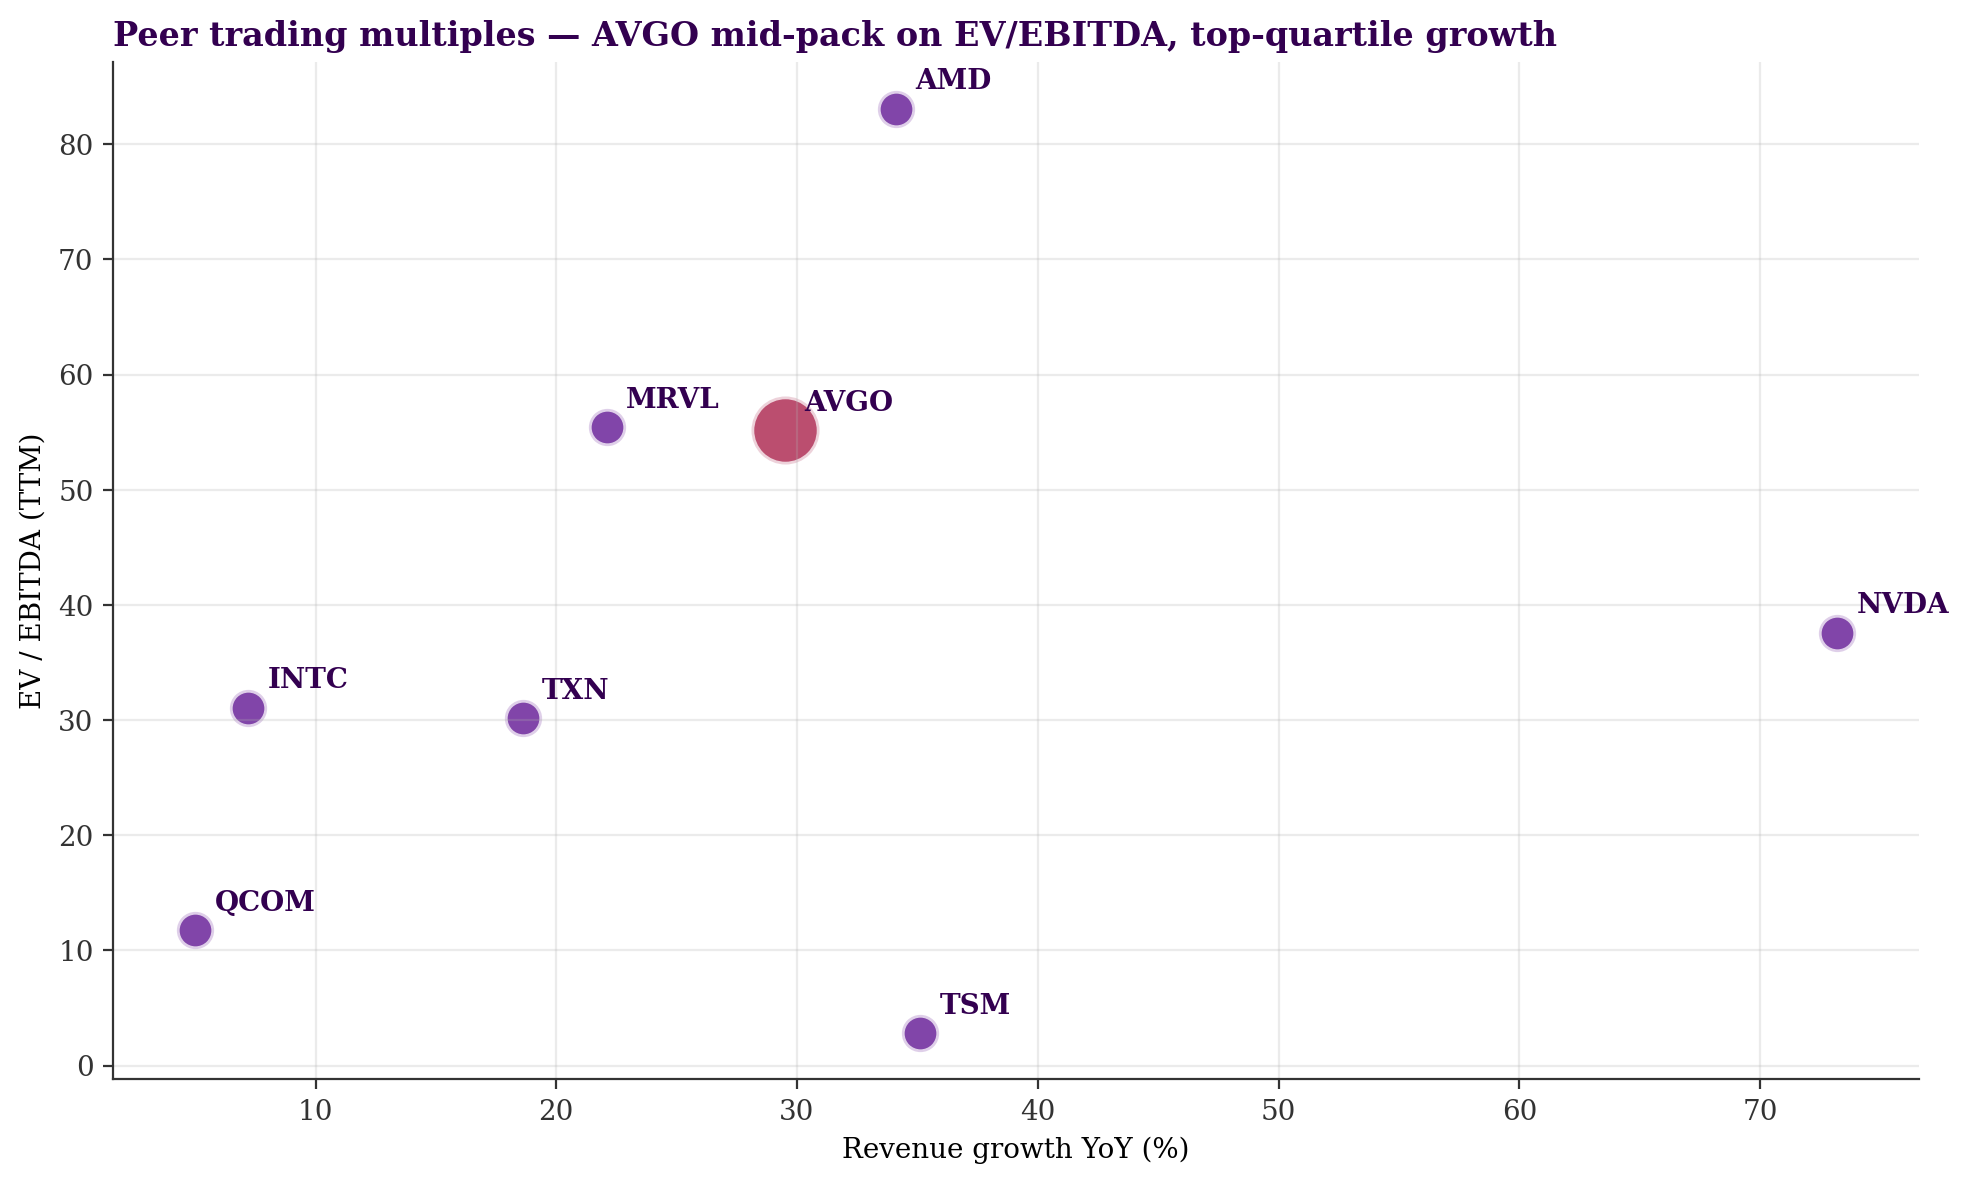
\includegraphics[width=\textwidth]{fig7_peers_scatter.png}
\caption{Peer scatter: AVGO mid-pack on EV/EBITDA, top-quartile on growth. Source: yfinance, team analysis.}
\end{figure}

\subsection{Monte Carlo simulation}

To capture distributional risk we run 10{,}000 paths sampling FY27 AI revenue (Normal, mean \$125B---calibrated to the Street consensus midpoint, sd \$25B), AI growth post-FY27 (mean 30\%, sd 10\%), terminal growth (mean 3.0\%, sd 0.5\%), WACC (mean base, sd 0.5\%), steady-state EBITDA margin (mean 68.5\%, sd 2.5\%), and capex/sales ratio (mean 1.1\%, sd 0.3\%). The resulting intrinsic-price distribution has:

\begin{table}[!ht]
\centering
\small
\begin{tabular}{p{4.0cm}rp{4.0cm}r}
\arrayrulecolor{nyuviolet}\toprule
Mean             & \$471 & 5th percentile  & \$287 \\
Median           & \$456 & 25th percentile & \$378 \\
Standard deviation & \$131 & 75th percentile & \$544 \\
Probability $>$ spot & \textbf{60.7\%} & 95th percentile & \$711 \\
\arrayrulecolor{nyuviolet}\bottomrule
\end{tabular}
\caption{Monte Carlo distribution statistics, 10{,}000 paths. Source: Team analysis.}
\end{table}

\begin{figure}[!ht]
\centering
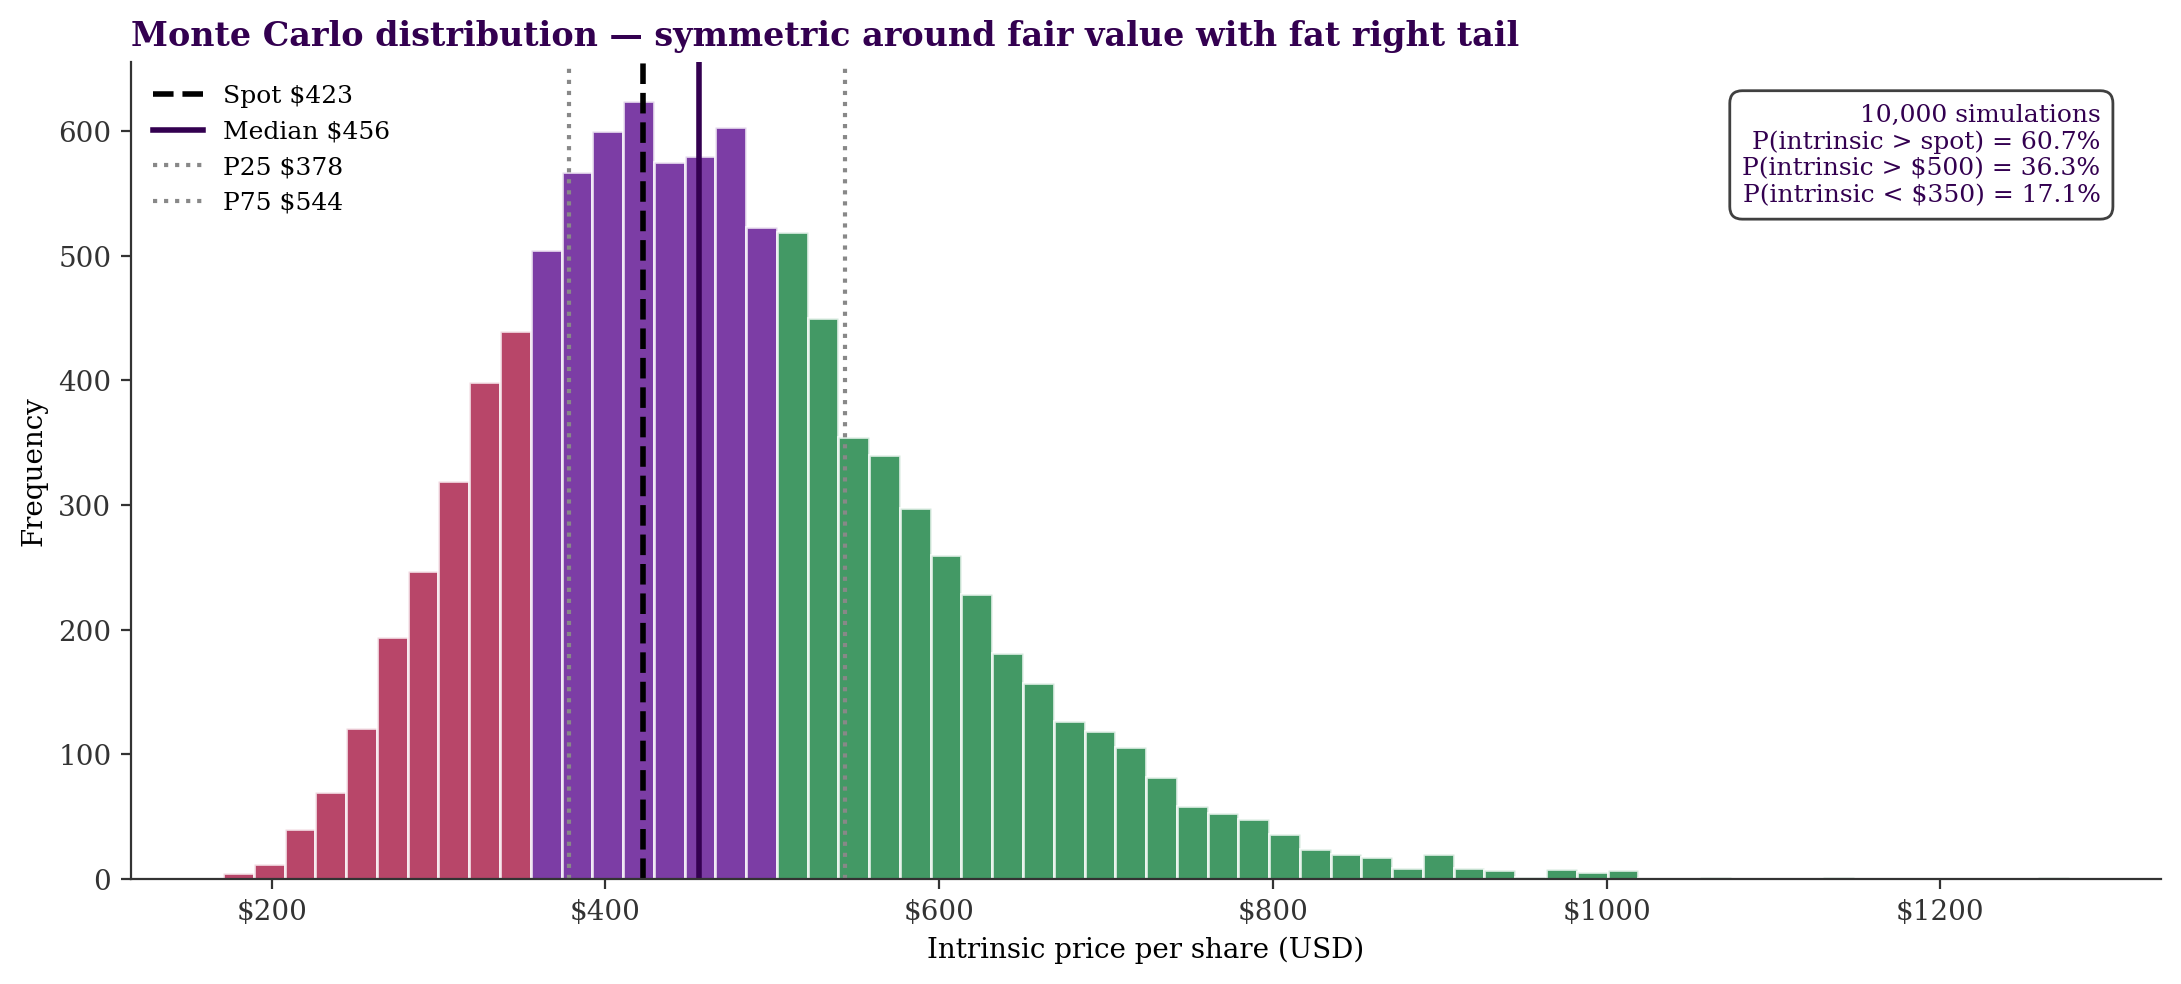
\includegraphics[width=\textwidth]{fig5_monte_carlo.png}
\caption{Monte Carlo intrinsic-price distribution. Source: Team analysis.}
\end{figure}

The 60.7\% probability that intrinsic value exceeds spot, combined with $E[\text{intrinsic}] = \$471$ vs.\ spot of \$423, supports our BUY rating.

\subsection{Football field synthesis}

\begin{figure}[!ht]
\centering
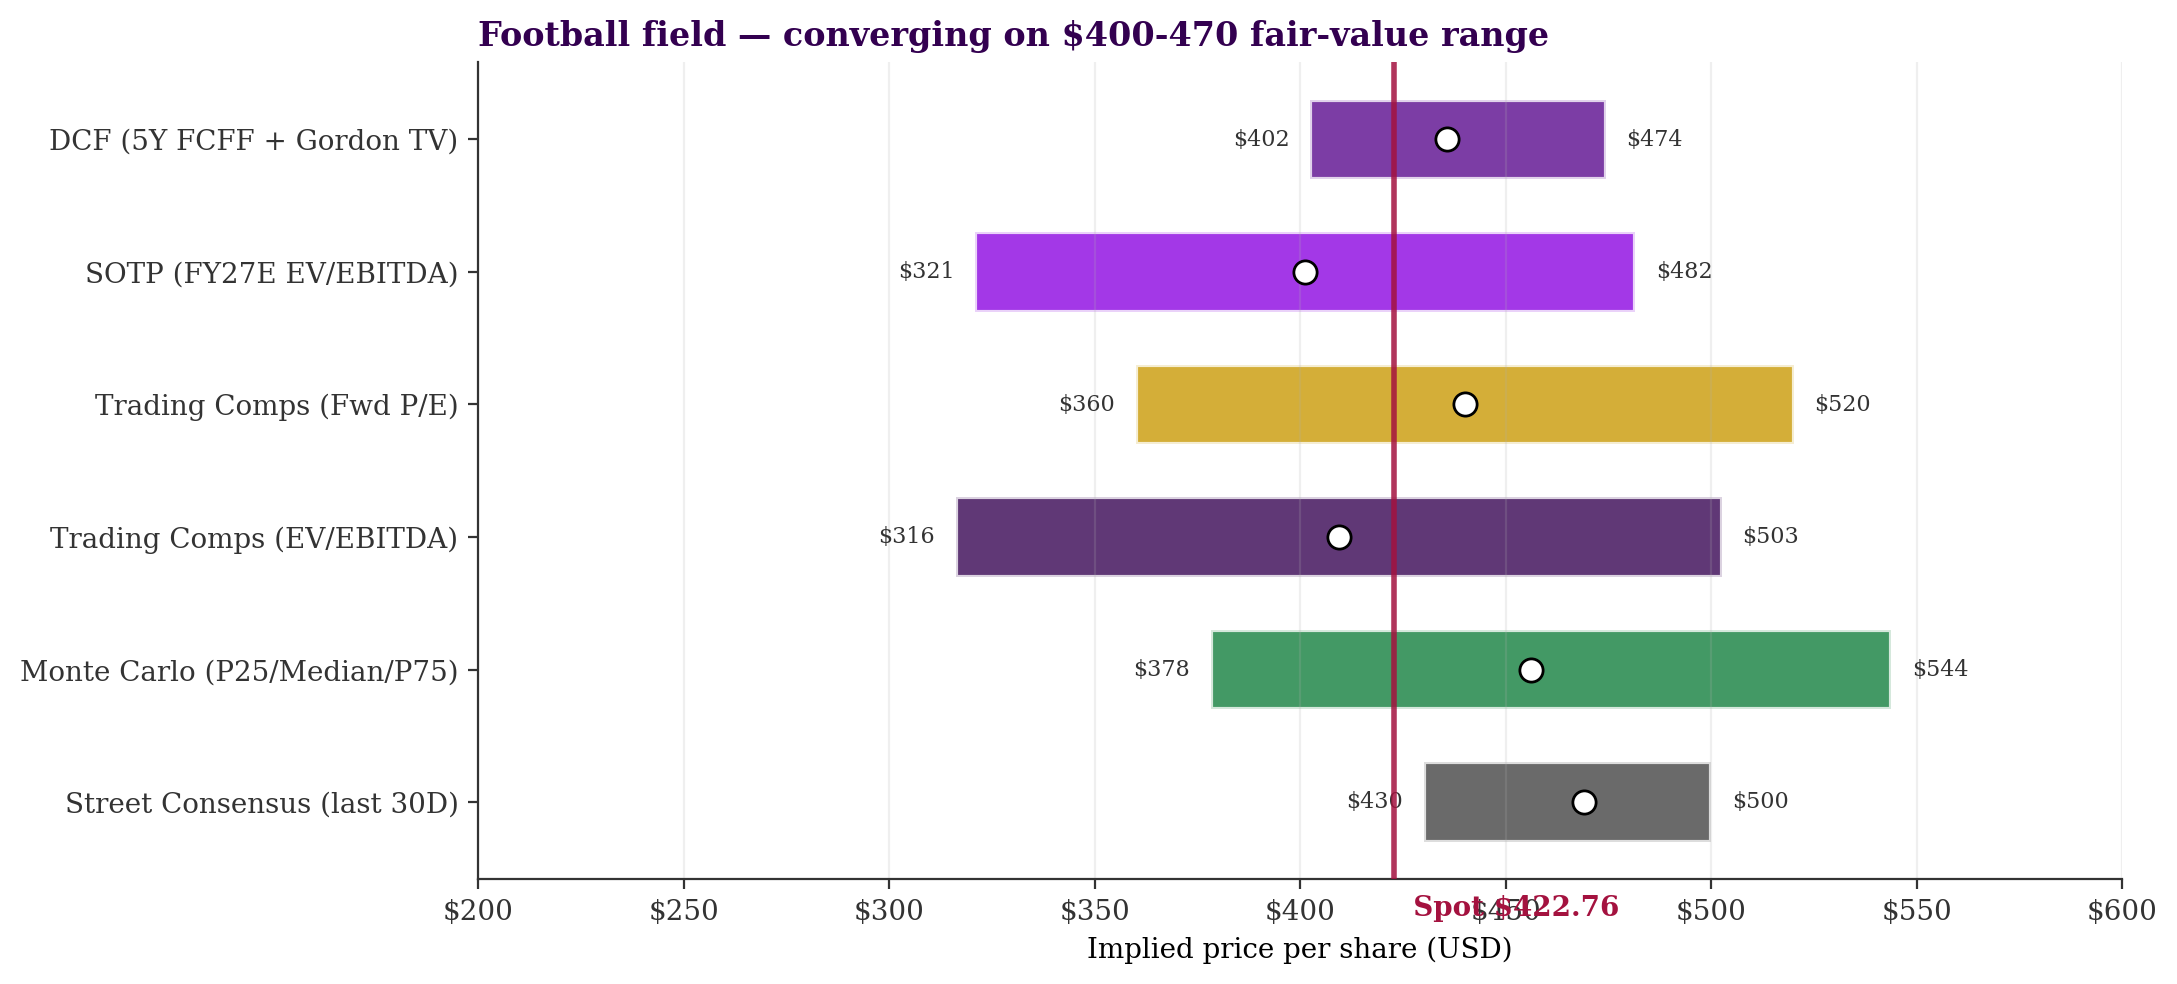
\includegraphics[width=\textwidth]{fig4_football_field.png}
\caption{Valuation football field. Source: Team analysis.}
\end{figure}

The methods cluster within a defensible \$400--\$510 range. Our December-2026 price target of \$475 sits at the Street median and roughly at the MC mean---a level consistent with FY27 AI revenue printing in the \$120--130B range (where management's ``\$100B+'' floor and Street upper-bound converge).

\newpage

% =============================================================================
% RISKS
% =============================================================================
\section{Risk Framework}
\sectionbyline{Lead author: Martin Baretto}{Risk lead}

We evaluate ten distinct risk factors against probability and equity-value impact:

\begin{figure}[!ht]
\centering
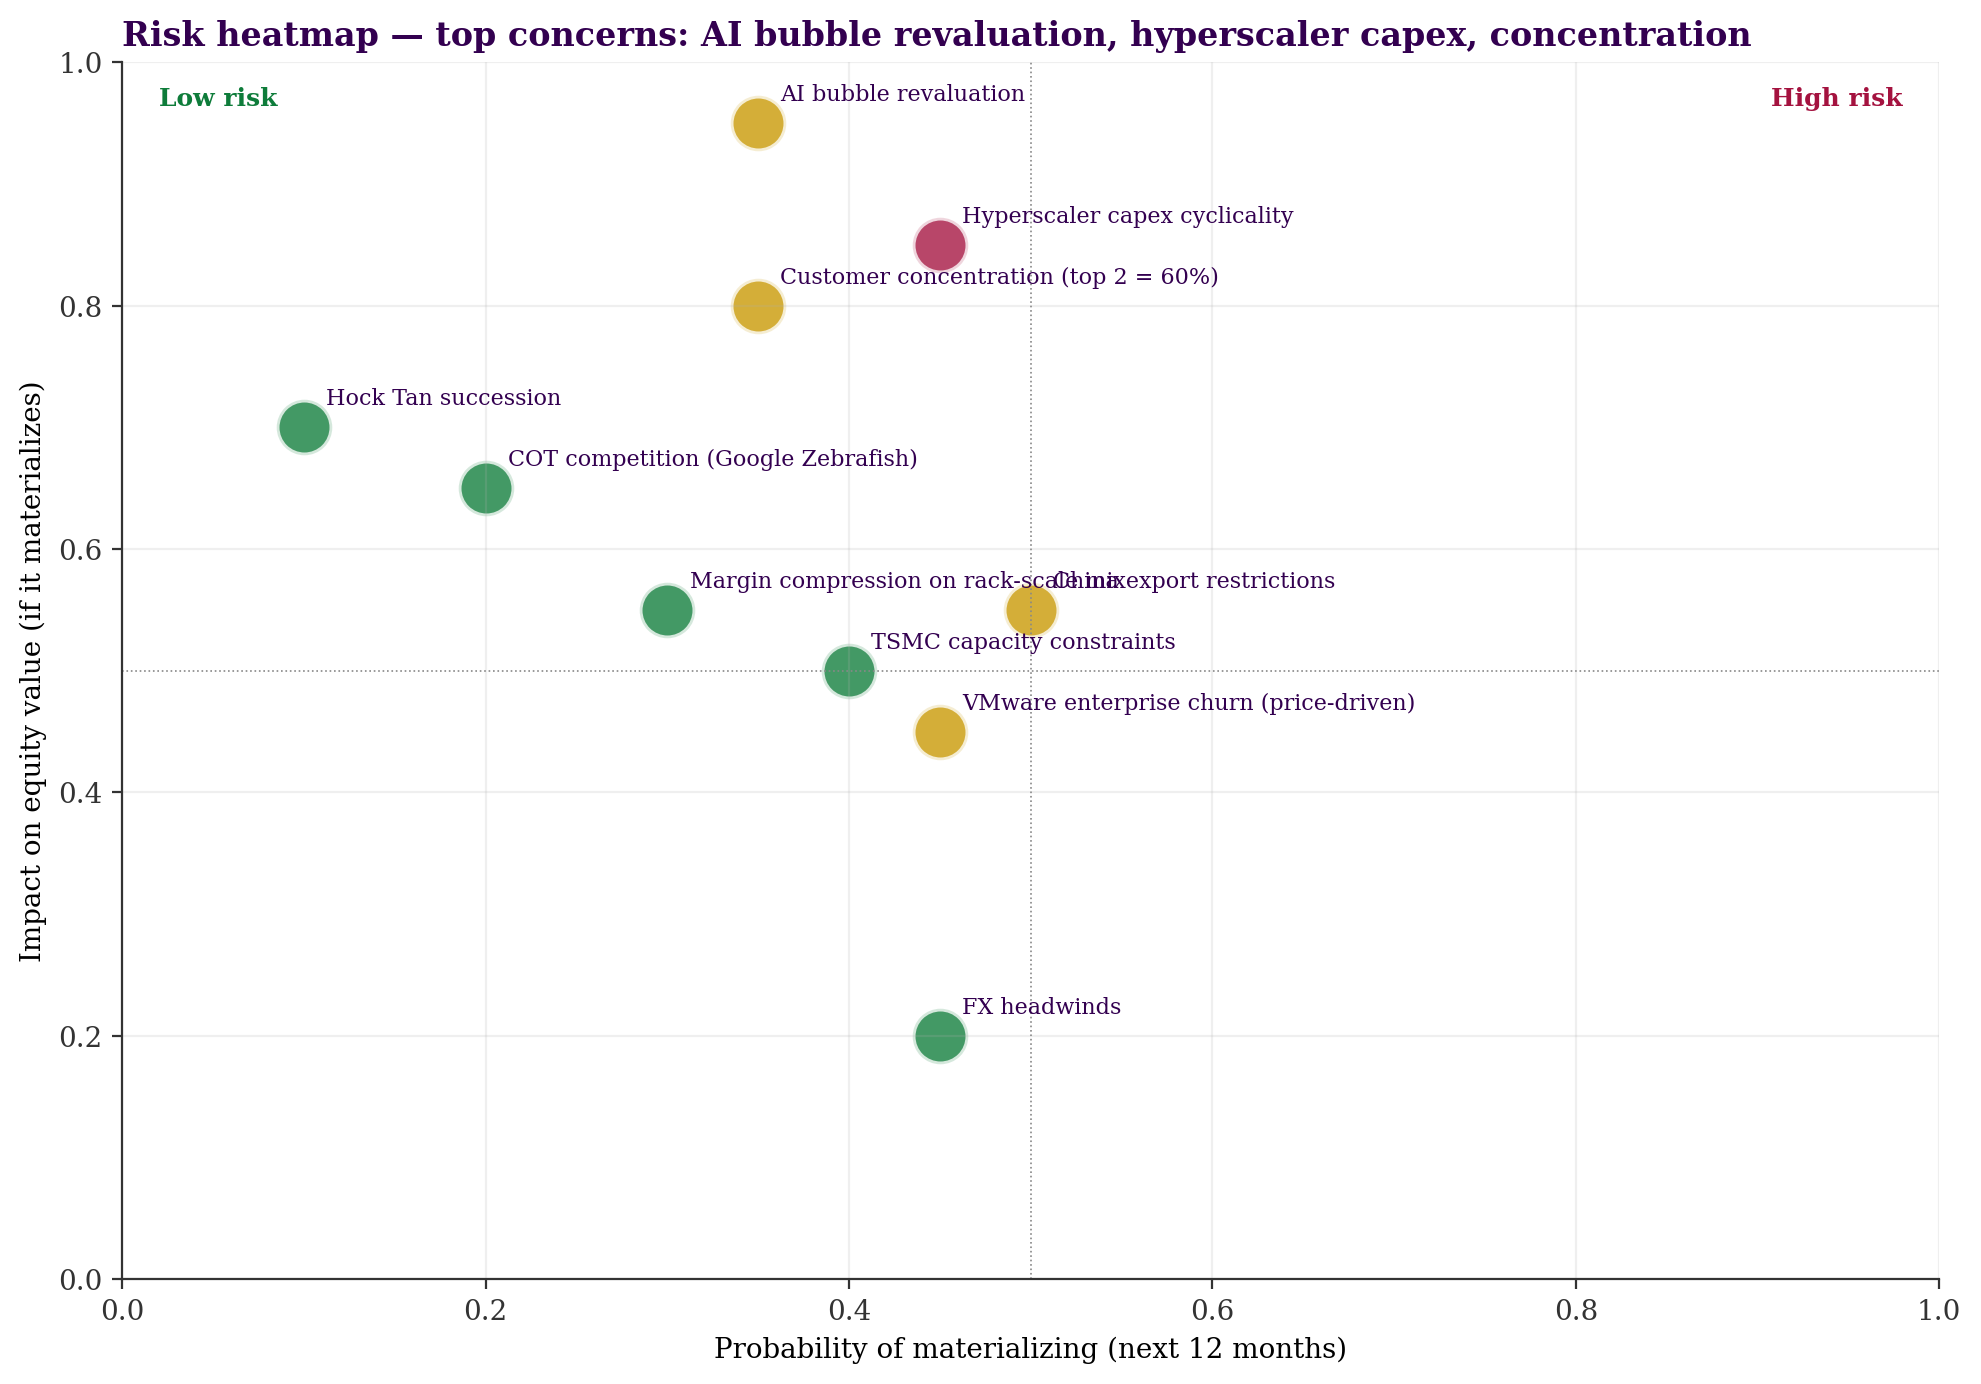
\includegraphics[width=\textwidth]{fig11_risk_matrix.png}
\caption{Risk heatmap. Source: Team analysis.}
\end{figure}

\subsection{High-probability, high-impact risks}

\begin{itemize}[leftmargin=*]
\item \textbf{Hyperscaler capex cyclicality (P=45\%, I=85\%).} Google, Meta, and Microsoft together represent the bulk of Broadcom's AI customer base. A coordinated capex pullback would compress 2027--28 revenue and the multiple. We model 30\% downside in our Monte Carlo bear case, consistent with the historic semiconductor cycle.
\item \textbf{Customer concentration (P=35\%, I=80\%).} Google + Anthropic represent $\sim$60\% of FY27E AI mix. Either renegotiation, share-loss to a COT alternative (Google Zebrafish), or a strategic shift would be material.
\item \textbf{AI bubble revaluation (P=35\%, I=95\%).} Multiple compression risk if AI infrastructure capex narrative breaks. Broadcom's terminal value is 80\% of EV, making it acutely sensitive to a derating.
\end{itemize}

\subsection{Medium-impact risks}

\begin{itemize}[leftmargin=*]
\item \textbf{China export restrictions (P=50\%, I=55\%).} Broadcom has limited direct China exposure but TSMC dependencies remain a vector.
\item \textbf{VMware enterprise churn (P=45\%, I=45\%).} Aggressive subscription pricing has alienated mid-market enterprise customers; the high-end segment has been more sticky. UBS expects software growth to decelerate from current LDD\% to MSD\% range.
\item \textbf{Margin compression on rack-scale mix (P=30\%, I=55\%).} Reversed by management in March 2026 but could re-emerge if rack mix accelerates faster than networking attach.
\end{itemize}

\subsection{Lower-probability risks}

\begin{itemize}[leftmargin=*]
\item \textbf{COT competition (Google Zebrafish, P=20\%, I=65\%).} JPMorgan estimates an 18-month design lead; Zebrafish first silicon expected late 1Q26, volume not before 2H27.
\item \textbf{Hock Tan succession (P=10\%, I=70\%).} CEO has been at the helm 20 years; no announced succession plan.
\item \textbf{TSMC capacity constraints (P=40\%, I=50\%).} Mitigated by management commentary that Broadcom has secured capacity through FY28.
\end{itemize}

\section{Catalyst Calendar}

\begin{table}[!ht]
\centering
\small
\rowcolors{2}{rowshade}{white}
\begin{tabular}{p{2.6cm}p{4.5cm}p{8.0cm}}
\arrayrulecolor{nyuviolet}\toprule
\rowcolor{nyuviolet}\color{white}\textbf{Date} & \color{white}\textbf{Event} & \color{white}\textbf{What to watch} \\
\midrule
5-Jun-2026  & Q2 FY26 earnings    & AI revenue actuals vs.\ \$10.7B guide; gross-margin trajectory \\
4-Sep-2026  & Q3 FY26 earnings    & First commentary on FY27 AI revenue framing \\
H2-2026     & TPU Sunfish (3nm) ramp & Volume signal; Anthropic deployment cadence \\
H2-2026     & OpenAI rack first deployments & Confirmation of \$3B FY26 / \$10B FY27 trajectory \\
Dec-2026    & Q4 FY26 / FY27 guide & Critical for valuation; \$100B+ FY27 AI revenue floor in focus \\
\arrayrulecolor{nyuviolet}\bottomrule
\end{tabular}
\caption{Forward catalyst calendar.}
\end{table}

\section{Conclusion}
\sectionbyline{Authors: Yadav, Baretto, Sriram}{Joint conclusion}

Broadcom is the second-most-important AI infrastructure stock in the world after Nvidia, with a defensible six-customer XPU franchise, dominant networking silicon, and a high-margin software runway from VMware. The operating story over the next 24 months is clear and likely to be impressive in absolute terms.

After a 121.6\% twelve-month run, our DCF, SOTP, and comps cluster at \$400--440, but our Monte Carlo (calibrated to the Street consensus FY27 AI midpoint of \$125B) gives a 60.7\% probability of upside vs.\ spot with $E[\text{intrinsic}] = \$471$. We initiate at BUY with a \$475 December-2026 price target, equivalent to 12\% upside and in line with the Street median (\$477). We would consider further upgrading our PT on a positive print to FY27 AI revenue scale at the December 2026 guide.

\vfill
{\footnotesize\color{nyugrey}\textbf{Sources cited.} Broadcom Inc.\ Q1 FY2026 8-K (4-Mar-26); Broadcom 10-K FY2025; JPMorgan Equity Research, H.\ Sur (5-Mar-26 \& 25-Jan-26); Mizuho Securities, V.\ Rakesh (4-Mar-26); UBS Equities, T.\ Arcuri (5-Mar-26); Wells Fargo Securities, A.\ Rakers (4-Mar-26); Deutsche Bank Research, R.\ Seymore (4-Mar-26); Barclays Research, T.\ O'Malley (5-Mar-26); Bloomberg Equity Demo Tearsheet (12-Mar-26); company investor relations releases; Yahoo Finance via \texttt{yfinance}; Damodaran NYU Stern (2025 implied ERP). Reports accessed via NYU Bobst Library and provided to author Tanishk Yadav.}\\[6pt]
{\footnotesize\color{accentred}\textbf{Disclaimer.} This report is a student-prepared educational exercise authored by NYU MSFE students. It is not investment advice, not a recommendation to transact in AVGO securities, and not for distribution. Data as of 24/25 April 2026.}

\end{document}
